\documentclass[12pt]{report}

\usepackage{hyperref}
\usepackage[all]{hypcap}
\usepackage{listings}
\usepackage{appendix}
\usepackage{amsmath, amsthm, amssymb}
\usepackage{amsfonts}
\usepackage{graphicx}
\usepackage{placeins}
\usepackage{url}
\usepackage{color}
\usepackage{fancyhdr}
\usepackage{rotating}
\usepackage{array}
\usepackage{threeparttable}

\hypersetup{
%    bookmarks=true,         % show bookmarks bar?
    unicode=false,          % non-Latin characters in Acrobat�s bookmarks
    pdftoolbar=true,        % show Acrobat�s toolbar?
    pdfmenubar=true,        % show Acrobat�s menu?
    pdffitwindow=false,     % page fit to window when opened
    pdfnewwindow=true,      % links in new window
    colorlinks=false,       % false: boxed links; true: colored links
    linkcolor=red,          % color of internal linksline-numbers
    citecolor=green,        % color of links to bibliography
    filecolor=magenta,      % color of file links
    urlcolor=cyan           % color of external links
}

\lstset{ 
language=C,                			% choose the language of the code
basicstyle=\footnotesize,       % the size of the fonts that are used for the code
showstringspaces=false,         % underline spaces within strings
numbers=none,                   % where to put the line-numbers
numberstyle=\footnotesize,      % the size of the fonts that are used for the line-numbers
stepnumber=1,                   % the step between two . If it's 1 each line will be numbered
numbersep=5pt,                  % how far the line-numbers are from the code
backgroundcolor=\color{white},  % choose the background color. You must add \usepackage{color}
showspaces=false,               % show spaces within strings adding particular underscores
showtabs=false,                 % show tabs within strings adding particular underscores
escapeinside={\%*}{*)}          % if you want to add a comment within your code
}
%% Define a new 'leo' style for the package that will use a smaller font.
\makeatletter
\def
\url@leostyle{%
  \@ifundefined{selectfont}{\def\UrlFont{\sf}}{\def\UrlFont{\small\ttfamily}}}

\makeatother
%% Now actually use the newly defined style.
\urlstyle{leostyle}

\begin{document}

\begin{titlepage}

\thispagestyle{empty}
\rule{0pt}{50pt}

\begin{center}
 	\huge{Time-memory-data \\cryptanalysis of \\the HiTag2 stream cipher}\\
 		\vspace{2.5cm}
 	\Large{Master thesis project}\\
 	\Large{\today}\\
\end{center}

\vspace{5cm}

\begin{center}
	\Large{Rajesh Bachani \\(s061332)}\\
\end{center}
\end{titlepage}

\newpage
\thispagestyle{empty}
\vspace*{11cm}
{\noindent Department of Mathematics}\\
{Technical University of Denmark}\\
{Matematiktorvet, Building 303}\\
{DK-2800 Kgs.~Lyngby, Denmark}\\
{Phone +45 45253031, Fax +45 45881399}\\
{instadm@mat.dtu.dk}\\
{www.mat.dtu.dk}

\newpage
\pagenumbering{roman}
\setcounter{page}{1}
\pagestyle{fancy}
\addcontentsline{toc}{chapter}{Preface}

\chapter*{Preface}

This thesis was prepared at the Department of Mathematics, the Technical University of Denmark in partial fulfillment of the requirements for acquiring the Master of Science degree in Computer Science and Engineering.

The thesis is based on the implementation and evaluation of tradeoff attacks on the HiTag2 stream cipher. Three important tradeoff parameters are considered including the time taken for the attack, memory required for precomputation and the length of output available from the stream cipher. The thesis presents cryptanalysis results for four different tradeoff attacks by varying these parameters for each attack. 

\vspace{20mm}
\mbox{}\hfill
\begin{minipage}[t]{80mm}
Lyngby, September 2008\\
 \\
Rajesh Bachani
\end{minipage}

\addcontentsline{toc}{chapter}{Acknowledgements}

\chapter*{Acknowledgements}


% abstract.tex (Abstract)

\addcontentsline{toc}{chapter}{Abstract}

\chapter*{Abstract}

There are always two naive ways of breaking a block cipher, if no known weakness exists in it. One is the brute force attack, which requires availability of tremendous computational speed in order to try all possible keys. Other is the precomputed ciphertext attack, which imposes huge requirements on memory for storing ciphertext corresponding to all possible keys. Considering these extreme requirements, a middle way was proposed by Hellman called time-memory tradeoff (TMTO) attack. This attack reduces the requirement of time and memory to feasible domains making it possible to break ciphers under normal computational speed and memory, like using personal computers. The tradeoff is realized by storing a limited number of ciphertexts in memory selected by precomputing the Hellman tables.

TMTO attacks were first proposed on stream ciphers by Babbage and Golic. The TMTO principle for stream cipher differs from that for block cipher due to the much different functional working between them. The goal in the Babbage-Golic attack is to find atleast one occurring value of the internal state while the keystream is generated. This is done by matching fixed length subsequences of the keystream with precomputed output of same length from states stored in memory. This forms the basic principle for tradeoff attacks on stream ciphers. 

In this thesis, we have implemented the Babbage-Golic attacks on the HiTag2 stream cipher. HiTag2 was a proprietary algorithm designed by Philips and kept secret until recently the algorithm was reverse-engineered from its silicon implementation. Two different attacks are mounted on this cipher based on different assumptions on the availability of keystream and their results are presented. 

Precomputation structure of the Hellman tables was modified by Biryukov and Shamir to apply on stream ciphers. They termed this attack as time-memory-data tradeoff (TMDTO) attack using Hellman tables. Further, an improvement of Hellman tables was proposed by Oechslin which reduces the attack time by a factor of two and considerably solves the problem of collisions in Hellman tables. The precomputation structure by Oechslin is called rainbow table. Later, Erguler and Anarim proposed modifications to the rainbow table in order to apply them on stream ciphers.

We have implemented both the TMDTO attacks using Hellman and rainbow tables on HiTag2. The parameters which define the table structures are varied for both the tables and the results are presented. Further, we make a brief comparison between the proposals by Biryukov-Shamir and Erguler-Anarim, allowing us to see the performance of both these table structures for the same parameters. The results from the subsequent experiments performed with this implementation show the advantage of rainbow table over Hellman tables.

\tableofcontents
\listoftables
\listoffigures
\pagebreak

%----------------------------------------------------%
% with this we ensure that the chapter and section
% headings are in lowercase.


\renewcommand{\chaptermark}[1]{%
\markboth{#1}{}}
\renewcommand{\sectionmark}[1]{%
\markright{\thesection\ #1}}
\fancyhf{} % delete current header and footer
\fancyhead[LE,RO]{\bfseries\thepage}
\fancyhead[LO]{\bfseries\rightmark}
\fancyhead[RE]{\bfseries\leftmark}
\renewcommand{\headrulewidth}{0.5pt}
\renewcommand{\footrulewidth}{0pt}
\addtolength{\headheight}{0.5pt} % space for the rule
\fancypagestyle{plain}{%
\fancyhead{} % get rid of headers on plain pages
\renewcommand{\headrulewidth}{0pt} % and the line
}
\pagebreak
\pagenumbering{arabic}
\setcounter{page}{1}
\chapter{Introduction}
\label{chapter:intro}

\indent \textbf{\textit{Summary.}} The introduction chapter deals with the basics of stream ciphers and explains the following in sequence: one-time pads, pseudo-random sequence generators and linear feedback shift registers. Then, the HiTag2 stream cipher is introduced: first with a brief background about the cipher and later with details about it's functional working. 

\section{Cryptography}

Cryptography is the mathematical science of protecting secret information by transforming it into a form which is illegible. Generally, the original information is called \textit{plaintext} while the transformed information is called \textit{ciphertext}. Once plaintext is transformed into ciphertext, the latter can then be sent over an insecure channel to its destination. At the destination, the reverse transformation takes place yielding back the original information. Transformation of plaintext to ciphertext is referred to as \textit{encryption}, while the reverse process is called \textit{decryption}. A secret information called \textit{key} is used in both encryption and decryption. The key can be compared with the key for locks used to keep items safe. If the key is lost, then the lock can be broken by the holder of the key and the item can be stolen. Similarly, if an attacker knows the cryptographic key he can know the plaintext by decrypting the ciphertext.  

This is just one application of cryptography in modern security systems, namely providing confidentiality to secret information; though it was this application with which the idea of cryptography was first conceived. Modern cryptography is also capable of providing message integrity (that a message has not been modified), authentication between two parties (the guarantee that we are talking with the expected party), non-repudiation (that a party cannot deny the fact that it has carried through a transaction, if it has really done so) and so on. 

In the late 19th century, Kerckhoff published a very important principle \cite{kerckhoff} which has become the basis of modern security systems using cryptography. He said that the security of a cryptographic encryption-decryption algorithm must rest solely in the secrecy of its key, not in the secrecy of the algorithm itself. In other words, while designing a security system with cryptography, all cryptographic algorithms must be openly published, while the only secret parameter should be the keys used by the algorithms. This helps in the cryptanalysis of the algorithms and weaknesses can be found out by researchers and cryptanalysts. Though this is a very important principle, still the design of security systems continue to be based on propreitary algorithms. More information on certain secret algorithms and successful reverse-engineering techniques is provided in section \ref{sec:hitag2-background}.

Two kinds of cryptosystems exist, depending on the manner in which keys are used: symmetric-key and asymmetric-key. In symmetric-key cryptography, a single key is shared between two communicating parties, such that one party encrypts plaintext using the shared key and the other party decrypts the received ciphertext using the same key. In such systems, the secrecy of the shared key becomes extremely critical. Also, if the number of parties grows, the number of keys required in the system becomes large, since each communicating pair would hold a different key. In addition, sharing keys between each pair requires secure key establishment protocols. 

Symmetric-key cryptography was the only known kind of encryption before 1976, when Diffie and Hellman introduced the concept of asymmetric-key cryptography \cite{diffie1976ndc} for the first time. In asymmetric-key cryptography, the encryption and corresponding decryption are performed with different keys. Every party holds two keys: one public and one private. If \emph{Alice} wants to send a message to \emph{Bob}, she will encrypt the plaintext with the public key of \emph{Bob}. At the other end, \emph{Bob} would decrypt this ciphertext using his private key. The public-private key pair are related, but it is unfeasible to determine \emph{Bob}'s private key from his public key. Since every party holds two keys, the total number of keys is reduced considerably when compared to symmetric-key cryptosystems. Also, no key establishment protocols are needed as the public keys are distributed through public channels.

Symmetric-key algorithms are further classified into two different types, based on the manner in which plaintext is used by the encryption algorithm. These are block ciphers and stream ciphers. Block ciphers divide the plaintext into blocks of data, and each block is then encrypted separately. The sizes of the input and output blocks are same, irrespective of the size of the key. Successive output blocks are then connected to each other in some way, depending on the mode of operation of the block cipher. \emph{DES} (data encryption standard) has been one of the most widely used block ciphers with block size of 64 bits and key size of 56 bits. \emph{DES} has been recently replaced by \emph{AES} (advanced encryption standard) as the approved standard, through a public competition which called for new block cipher designs to replace \emph{DES}.

Stream ciphers on the other hand, have a different functional structure and working. Stream ciphers consist of an internal state, which is used in deriving one output bit through an output function. The internal state changes over successive clock cycles using an update function, consequently producing a stream of bits at the output. Bits of the plaintext are picked up in sequence and then \emph{xor}'ed bitwise with the output bits of the stream cipher to produce the ciphertext bits. The working of stream ciphers is explained in much detail in section \ref{sec:stream-cipher}. 

\section{Stream cipher}
\label{sec:stream-cipher}

\subsection{One-time pads} 
\label{sec:one-time-pads}

Before we explain the working of stream ciphers, it is important that we understand the motivation for the design of stream ciphers. An inspiration behind practical stream ciphers of today has been the one-time pad, which is also known as the Vernam cipher. In the one-time pad, the length of the key is required to be equal to or greater than the length of the plaintext. Each plaintext bit is operated with the corresponding key bit using the \emph{exclusive-or} (or \emph{xor}) operation, thus resulting in one bit of the ciphertext. So, if $p_i$ represents the $i^{th}$ bit of the plaintext, and $k_i$ represents the $i^{th}$ bit of the key, then the $i^{th}$ bit of the ciphertext is given by $c_i$ = $p_i \oplus k_i$. The corresponding decryption takes place as $p_i$ = $c_i \oplus k_i$. This is shown in the figure \ref{fig:one-time-pad}.

\begin{figure}[ht!]
	\centering
		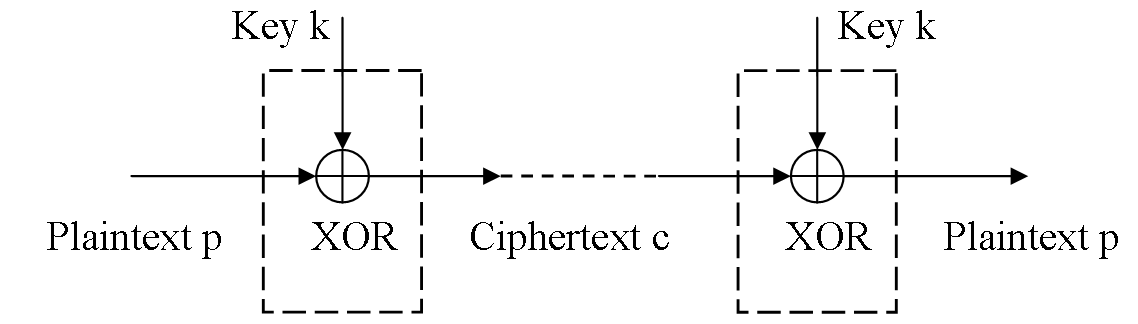
\includegraphics[width=4.4in]{./figures/one-time-pad.PNG}
	\caption{One-time pads}	
	\label{fig:one-time-pad}
\end{figure}

The key bits are required to be completely random, without any statistical correlation between them. With this pre-condition, there is no way that an adversary could determine the secret key just by knowing the ciphertext. Since the key bits are derived from a truly random source, there could be several combinations of the plaintext and the key which result in the given ciphertext. The attacker would, in such a scenario, never be able to determine which of the specific combination is the right one, even with infinite computing power at hand \cite{one-time-pads-link}.

If the attacker knows certain bits of the plaintext, then the corresponding bits of the key can be determined. If the key is not truly random, the attacker can predict some of the remaining bits of the key and thus decipher the remaining plaintext. Hence, the key should be truly random. 

Shannon in 1949, used his notion of information theory to formally prove that one-time pads are unbreakable \cite{shannon1949cts}, and termed them as having perfect secrecy. But for practical purposes, one-time pads have several weaknesses. These are explained in the following two points.
\begin{itemize}
\item The length of the key has to be equal to the length of the plaintext so that all the plaintext bits are encrypted. Thus to encrypt a long plaintext, large number of `random' key bits need to be generated. Managing such a huge set of key bits is not practical, since the storage and transfer need to be carried out securely. 

\item As the name of one-time pad suggests, a key can be used for just one transaction. If the same key is used for encrypting two different plaintext messages, the chances that the key being broken are extremely high. These chances are precisely zero when the key is used just for one encryption and is derived from a true random source. So it is suggested that a previous key not be used again.
\end{itemize}

Considering the above points, rather than transmitting the key then, it is a better idea to transmit the plaintext itself through the secure channel. Clearly, one-time pads are not good enough for being deployed in practical systems, but they reveal a strong design basis for stream ciphers. The component missing between one-time pads and stream ciphers is the pseudo-random sequence generator, which is discussed next. 

% still, one-time pad is useful. explain. 

\subsection{Pseudo-random sequence generators}
\label{sec:psrg}

Pseudo-random sequence generator (PRSG) is used to derive a seemingly random sequence of bits called the \emph{keystream}, using a small initial seed value. PRSG's are finite state machines having an internal state, which is initialized using the secret key, along with some more initialization parameters if required. A PRSG uses the following two functions internally.
\begin{itemize}
\item A linear \emph{update function} is used to derive the next state using the current state.
\item A linear or non-linear \emph{output function} is used to generate an output bit from the current state. 
\end{itemize}

\begin{figure}[ht!]
	\centering
		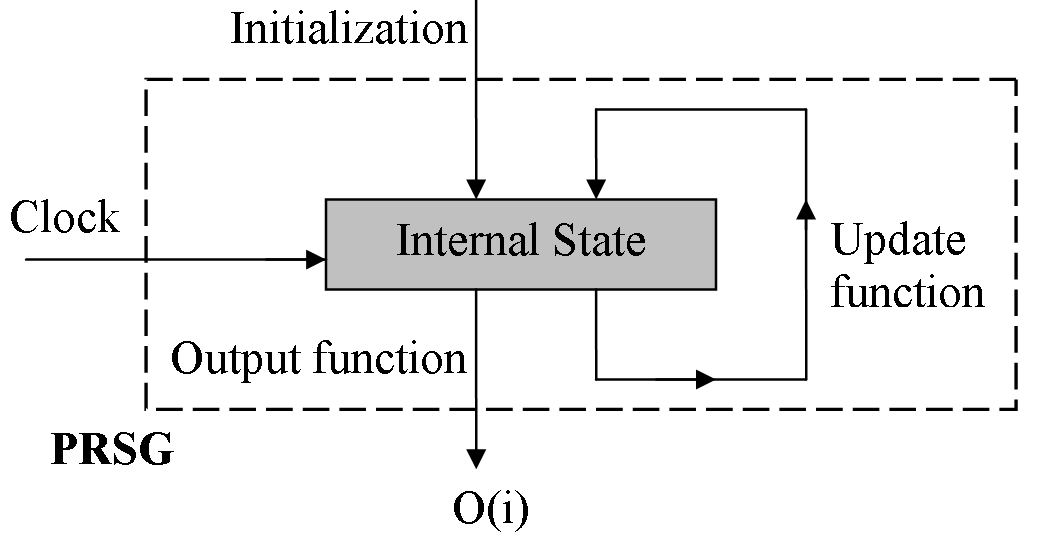
\includegraphics[width=3.5in]{./figures/prsg.PNG}
	\caption{Internal model of Pseudo-random sequence generator}	
	\label{fig:prsg}
\end{figure}

Figure \ref{fig:prsg} shows the internal model of a PRSG. A stream of the output bits (occuring as the PRSG changes states in every clock cycle) constitutes the keystream. It is important to note that the keystream is not truly random, but as the name of the generator suggests, it is pseudo or seemingly random. 

\paragraph{\textit{Use in stream cipher construction.}}
\label{para:stream-construction} 
We need to use secret keys of fixed length independent of the length of plaintext, in the construction of stream ciphers. Typically the key lengths are 128, 256 or 512 bits, which are considered secure by the standards of the computational power existing today. 
% NEEDED - check this and need a reference here %
The small secret key is used in the initialization of the PRSG thus generating a long keystream which replaces the long secret key in the one-time pads. The trade-off here is that the keystream is not truly random. As a result, the perfect secrecy of one-time pads does not apply to stream ciphers, but at the same time, the strength of the pseudo-random sequence generator becomes extremely important in determining how strong the stream cipher is cryptographically.

An overview of a stream cipher design is shown in figure \ref{fig:stream-cipher}. The secret key and other initialization parameters like initialization vector (IV) etc. are used to initialize the internal state. Once the initial state is prepared, the PRSG is ready to generate the keystream. Bits of the plaintext are \emph{xor}'ed along with corresponding bits from the keystream to generate a stream of encrypted bits. In effect, the plaintext and the keystream are used to produce the ciphertext.

\begin{figure}[ht!]
	\centering
		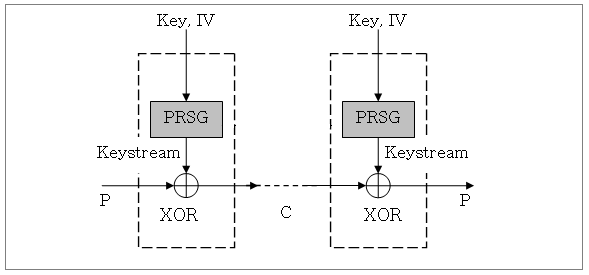
\includegraphics[width=3in]{./figures/stream-cipher.PNG}
	\caption{Deployment of PRSG in a stream cipher}	
	\label{fig:stream-cipher}
\end{figure}

At the receiver end, the PRSG is initialized using the same parameters. Any change in the initialization results in the generation of a different keystream leading to incorrect decryption of the received ciphertext. With the correct keystream, ciphertext is decrypted giving the correct plaintext. 

% security of PRSG %
As briefly mentioned before, the security of the stream cipher much depends on the security properties of PRSG. The output sequence is required to behave as a true random sequence. One very important consideration in ascertaining adequate security \cite{robshaw1995sct} is mentioned below.

The period of the keystream should be large. This becomes extremely important when the length of the plaintext is large. If the keystream repeats, the same sequence would encrypt different parts of the plaintext. If the attacker has knowledge of some initial part of the plaintext, then the initial keystream encrypting the known plaintext can be recovered. This initial keystream can later be used to decrypt part of the ciphertext which the attacker does not know. Even if the attacker has no knowledge of plaintext, certain properties of the plaintext can be derived from the two ciphertexts encrypted using the same keystream. 

On the other hand, the requirement on how large the period should be depends on the amount plaintext expected to be encrypted.

\subsection{Linear feedback shift registers} 
\label{sec:lfsr}
The most widespread implementation of PRSG's is done using a linear feedback shift register (LFSR). Other methods for generating pseudo-random sequences exist as well. Since we are mainly going to deal with an LFSR based generator (HiTag2) in this thesis, we would describe only them here. Other methods of generating pseudo-random sequences are linear congruence generators and non-linear feedback shift registers. For an introduction to these methods, we point to \cite{zeng1991pbg}. 
% reason why LFSR are widely used, and why are we more interested in them %
% more info on other generators %

It is important to note that LFSR constitutes only the \emph{update function} of the PRSG. The \emph{output function} of the PRSG needs to be implemented on top of the LFSR. An LFSR consists of two important components which are a shift register and a linear feedback function.\\

\textbf{\emph{Shift Register.}} A shift register holds a fixed number of bits, and shifts each of them into corresponding adjacent positions (all in a particular direction) on every clock cycle. If the direction of the shift is taken to be rightwards, then in every clock cycle there is a new bit on the leftmost position of the register, and the rightmost bit is excluded from the register, as shown in the figure \ref{fig:shift-register}. If the $n$ bits of the shift register are represented by $s_{n-1}$, $s_{n-2}$, $\ldots$ , $s_{1}$, $s_{0}$, then on every clock cycle we have the following transformations: $s_{out}$ = $s_{0}$, $s_{0}$ = $s_{1}$, $\ldots$, $s_{n-2}$ = $s_{n-1}$, $s_{n-1}$ = $s_{in}$; where $s_{out}$ is the bit which is excluded from the register and $s_{in}$ is the new bit. The application implementing the shift register decides how the $s_{in}$ and $s_{out}$ bits are handled.

\begin{figure}[ht!]
	\centering
		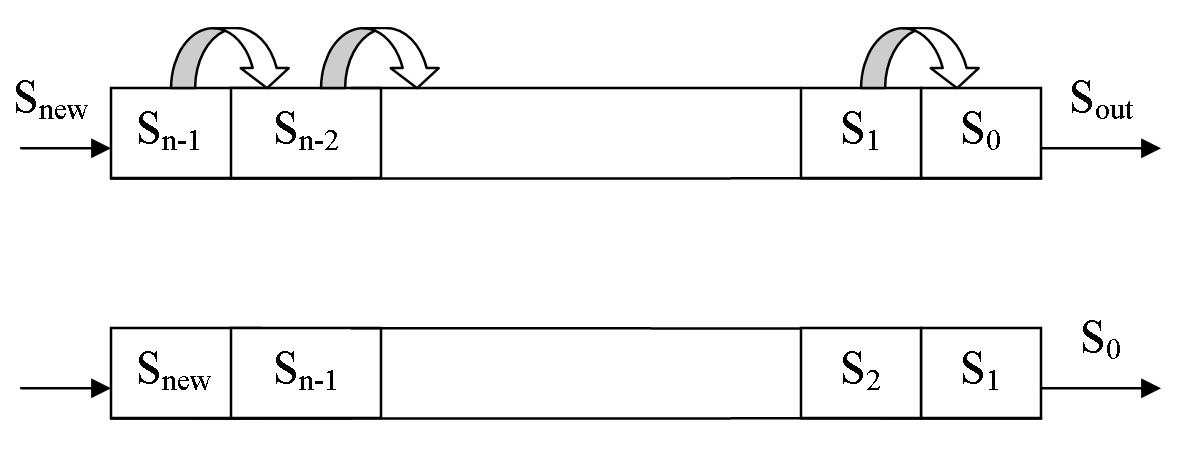
\includegraphics[width=4in]{./figures/shift-register.PNG}
	\caption{A simple shift register and its state after one clock cycle}	
	\label{fig:shift-register}
\end{figure}

For example, one of the uses of shift registers has been in the conversion of sequential (or serial) data to parallel data, and vice versa \cite{lfsr-link}. A sequence of bits can be stored in the shift register over a period of $n$ clock cycles, and retrieved in a parallel form in the $(n+1)$'th clock cycle. Hence, $s_{in}$ bit is taken from the input sequential stream, while $s_{out}$ bit is not used. 

For parallel-to-sequential data conversion, a parallel stream of $n$ bits is stored in the shift register in one cycle, and retrieved sequentially over the next $n$ clock cycles. The bit $s_{in}$ is not used in this case and $s_{out}$ stores bits of the sequential output stream.\\

\textbf{\emph{Linear feedback.}} A \textit{feedback function} defines the $s_{in}$ bit as a function of one or more bits from among the $n$ bits of the shift register. If the function is \textit{linear}, it said to be a \textit{linear feedback function}. Linearity is incorporated in the design generally by the use of $xor$ as the feedback function. Other boolean functions which are linear are negation, logical biconditional, tautology, and contradiction. According to the Wikipedia page on linearity \cite{linear-wiki}, 
\begin{quote}
\footnotesize{A Boolean function is linear if (1) In every row of the truth table in which the value of the function is `T', there are an even number of `T's assigned to the arguments of the function; and in every row in which the truth value of the function is `F', there are an odd number of `T's assigned to arguments; or (2) In every row in which the truth value of the function is `T', there are an odd number of `T's assigned to the arguments and in every row in which the function is `F' there is an even number of `T's assigned to arguments.
}
\end{quote}

The above properties can be easily checked to hold in the truth table of the \emph{xor} function.

A simple example of an LFSR is shown in figure \ref{fig:lfsr-example1}. Let us examine the linear feedback function more closely for this example. As can be seen, certain selected bits from the shift register are \emph{xor}'ed, and the resulting value is assigned to the leftmost bit, but only in the next clock cycle (in addition to the shifting of bits). As a result, the internal state of the LFSR is changed. If we number the bits from \emph{1, 2,} $\ldots$ , and so on, then the bits 11, 13, 14 and 16 are used in the feedback function. These bits are referred to as \emph{tap sequence} or $taps$ of the LFSR. In general, the outputs that affect the input of the LFSR are called $taps$.\\


\begin{figure}[ht!]
	\centering
		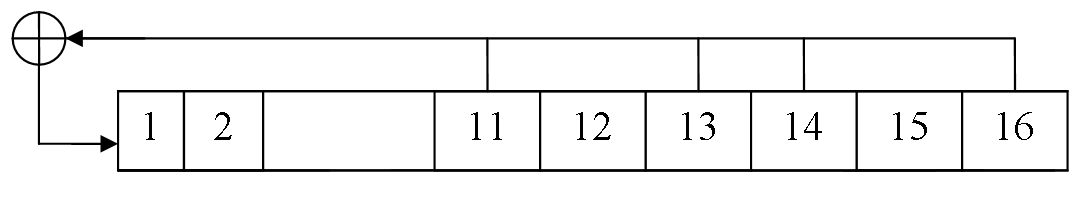
\includegraphics[width=4in]{./figures/lfsr-example.PNG}
	\caption{A simple LFSR of size 16 bits and tap bits 11, 13, 14 and 16}	
	\label{fig:lfsr-example1}
\end{figure}

\noindent \textit{\textbf{Maximal length tap sequence.}} Depending on the initial state, the LFSR runs through a set of states and then returns back to the initial state. This forms a cycle of states. In order to use the LFSR for generating a pseudo-random sequence, we want to have the longest cycle of the LFSR states. In other words, we want the LFSR to traverse through all possible states, which is equal to $2^n$, where $n$ is the number of bits in the shift register. This is important since it is desired that the pseudo-random sequence has a large period, as mentioned in the requirements for PSRG in section \ref{para:stream-construction}.

It is important to note that if the LFSR is in a state where all the bits are \textbf{0}, then the next state would also be the same. This condition occurs because the \textit{xor} of any number of \textbf{0}'s is always \textbf{0}. Such a state is called the \textit{trivial state}. As a result, no cycle is formed if the initial state is the trivial state. Hence the maximum number of different states in the LFSR becomes $2^n-1$. A tap sequence which generates the particular cycle of states such that the period of the LFSR is $2^n-1$, is called the maximal length tap sequence. 

The tap sequence for the LFSR in figure \ref{fig:lfsr-example1} is a maximal length tap sequence. In order to verify maximal length tap sequences, the polynomial representation of the tap sequence is considered.\\

\noindent \textit{\textbf{Polynomial representation of tap sequence.}} Once we have a tap sequence, we can express it in the form of a polynomial with modular \textbf{2} coefficients. For the example shown in figure \ref{fig:lfsr-example1}, the polynomial representation of the tap sequence is

\begin{center}
$p(x)$ =  1 + $x^{11}$ + $x^{13}$ + $x^{14}$ + $x^{16}$
\end{center}

The powers of $x$ represent the tap bits. The \textbf{1} in the starting is a result of $x^0$ and represents the $s_{in}$ bit, since $s_{in}$ can be interpreted to exist at the \textbf{0}'th position of the shift register (this existence is just theoretical). A given tap sequence is a maximal length tap sequence if the polynomial representing it is irreducible i.e.~the polynomial cannot be factored into nontrivial polynomials.

It is important to note that the polynomial representation should not depend on the numbering of the bit positions. If the same LFSR is numbered in the fashion as shown in figure \ref{fig:lfsr-example2}, then we have the following polynomial representation.
\begin{align*}
p'(x) &= x^{17} + x^{6} + x^{4} + x^{3} + x
\end{align*}
\begin{align}
\label{eq:poly-1} p'(x) &= x*(x^{16} + x^{5} + x^{3} + x^{2} + 1)\\
\label{eq:poly-2} p'(x) &= x^{16} + x^{5} + x^{3} + x^{2} + 1
\end{align}

\begin{figure}[ht!]
	\centering
		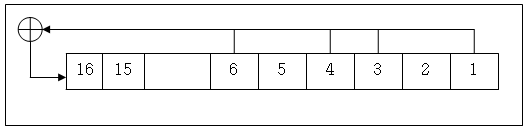
\includegraphics[width=4in]{./figures/lfsr-example-reverse.PNG}
	\caption{A different numbering of the bit positions for the same LFSR}	
	\label{fig:lfsr-example2}
\end{figure}

The ploynomial in equation \ref{eq:poly-1} is irreducible only if the term $(x^{16} + x^{5} + x^{3} + x^{2} + 1)$ is irreducible, so we rewrite $p'(x)$ after ignoring the factor $x$ in the equation. Since both $p'(x)$ and $p(x)$ represent the same LFSR, they should be related in some way. The Wikipedia page for LFSR at \cite{lfsr-wiki} states the following in this context,

\begin{quote}
\footnotesize{
Once one maximal tap sequence has been found, another automatically follows. If the tap sequence, in an $n$ bit LFSR, is [n,A,B,C,0], where the \textbf{0} corresponds to the $x^0$ = 1 term, then the corresponding `mirror' sequence is [n,n-C,n-B,n-A,0].}
\end{quote}

In our example, the tap sequence [16,14,13,11,0] has a mirror tap sequence [16,5,3,2,0], which are represented by the polynomials $p(x)$ and $p'(x)$.

Hence, the choice of an appropriate polynomial for the LFSR is important in order to guarantee that the LFSR moves through all the possible internal states before the first state repeats.

%
% NEEDED - \subsection{Some stream ciphers}
%

\section{The HiTag2 stream cipher}
\label{sec:hitag2}

\subsection{Background}
\label{sec:hitag2-background}
HiTag2 is a stream cipher originally designed by Philips Semiconductors (now NXP Semiconductors) and used for mutual authentication between a car remote control and controller in the car. Such systems (called remote keyless entry or RKE systems) have been widely implemented in modern electronic cars, and facilitate unlocking of car doors upon just a button press from within a certain maximum distance from the car. The HiTag2 stream cipher provides two-way authentication, authenticating the two entities to each other one by one. In such a protocol, a nonce is sent across from the initiator to the responder. The responder initializes the stream cipher using the nonce as IV, additionally using the secret key and its fixed ID. Some fixed length of the keystream is then sent back to the initiator as authenticator. The similar protocol is executed to authenticate the initiator to the responder. 

But, this is just one use of the cipher, and other applications could use the cipher for authentication as well as encryption. If hiding the plaintext is desired, the message bits are \emph{xor}'ed with the keystream bits before sending them over the public channel. 

HiTag2 was kept secret by Philips until it was reverse-engineered using the cipher's software implementation. The microcode (or assembly code) of HiTag2 was decompiled from the implementation available in the car remote controls and the RKE receivers. The C code for the cipher is availabe on the website \cite{hitag2-code}. A full system level specification of the RKE system by Philips (titled Active Tag and IC) implementing the HiTag2 cipher is also available \cite{active-tag-datasheet}. HiTag2 now is the intellectual property of NXP, but the specification document holds the name of Philips since NXP did not come into existence at that time in 2005. Also, since the cryptography (HiTag2) on the RKE system was kept secret at that time, HiTag2 modes are just mentioned without any further information on the functional working of the cipher.

The design of HiTag2 is very similar to a recently reverse-engineered \cite{NohlESP-2008-usenix} stream cipher called Crypto-1, which is used in Mifare Classic smartcards by NXP. The Mifare family comprises of contactless smart cards and card readers, with a variety of different features including memory availability on the cards to store data and read/write permissions on the cards. As a result of these features, Mifare system is widely used in applications requiring more than just authentication. Some such applications are ticketing system for public transportation (OV-Chipkaart in Netherlands, Oyster cards in UK etc.) and access control in buildings. Crypto-1 cipher used in Mifare Classic cards and readers was proprietary until recently when Nohl et al.~\cite{NohlESP-2008-usenix} reverse-engineered the algorithm from its silicon implementation.

In addition, the same Mifare Classic cards and readers are shown to be easily clonable \cite{dekoninggans2008pam} by researchers at Radboud University. They have analyzed the communication protocol between the card and the reader, and have been been able to show that the there are several weaknesses in the Crypto-1 cipher. They have been able to recover the necessary keystream by analyzing the protocol messages. The details of this protocol analysis complements the work by Nohl et al., and using both the ideas, mounting brute-force attack on the cipher has been made possible. 

Apart from reverse-engineering from software or hardware implementations, a black-box reverse-engineering has also been applied to break secret algorithms. The DST RFID tag (using the DST stream cipher) was broken in 2005 using black-box reverse-engineering \cite{bono2005sac}, i.e.~by selecting certain input formats and using both the input and output combinations to deduce the structure and working of the cipher. The most common application of Texas Instrument's DST tag is in vehical immobilizer systems and electronic payment systems \cite{dst-rfid-analysis}. 

In the next section, the working of HiTag2 is described.

\subsection{Cipher Description}
The basic components of the HiTag2 stream cipher are outlined below.
\begin{itemize}
\item 48 bit key
\item 32 bit serial ID
\item 32 bit initialization vector (IV)
\item 48 bit internal state with linear update function (basically, an LFSR)
\item Non-linear output function based on multiplexor, with data bits being constant and address bits depending on the current internal state
\end{itemize}

The entire setup of the keystream generator is done in two phases. The first phase is the initialization of the LFSR, which sets the internal state to a non-zero value using the key and the serial ID. The second phase is the setup of the LFSR during which the LFSR is clocked (resulting in the shifting of bits) using the key and IV bits in the process. Once the LFSR is set, the keystream is ready to be generated from the internal state right away. We describe these phases in detail here.\\ 

\noindent \textit{\textbf{1. LFSR Initialization.}} The initialization step of the LFSR is straightforward. Instead of initializing the LFSR with random bits, the serial ID and an initial part of the key are used. The 32 bits of the serial ID are stored in the least significant 32 bits of the LFSR (bits from index 0 through index 31). Then, the least significant 16 bits of the key are stored in the remaining 16 bits of the LFSR (bits from index 32 through index 47), as shown in figure \ref{fig:hitag2-1}. With this the initialization of the LFSR is complete.\\

\begin{figure}[ht!]
	\centering
		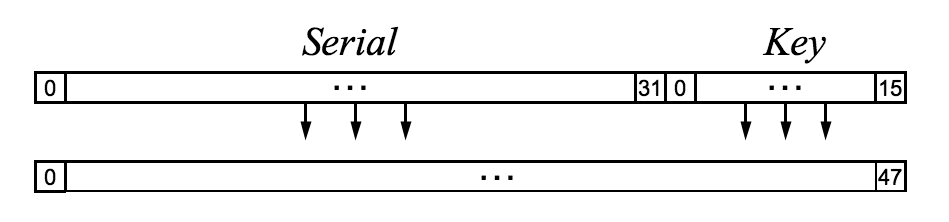
\includegraphics[width=4.3in]{./figures/hitag2-1.PNG}
	\caption{LFSR Initialization \cite{hitag2-figure}}	
	\label{fig:hitag2-1}
\end{figure}

\noindent \textit{\textbf{2. LFSR Setup.}} During the setup of the LFSR, the 32 bits of IV are used with the remaining 32 bits of the key. The bits in the LFSR are shifted to the right in every clock cycle, and a new value is stored in the leftmost bit. In every clock cycle, an xor of the following three bits is computed: one bit from the key (range: bits from index 16 through 47), one bit from the IV (range: bits from index 0 through 31) and the output bit from the non-linear output function. The computed bit is stored at the leftmost bit of the LFSR. After 32 clock cycles, the internal state is prepared for keystream generation. This is shown in figure \ref{fig:hitag2-2}.\\

\begin{figure}[ht!]
	\centering
		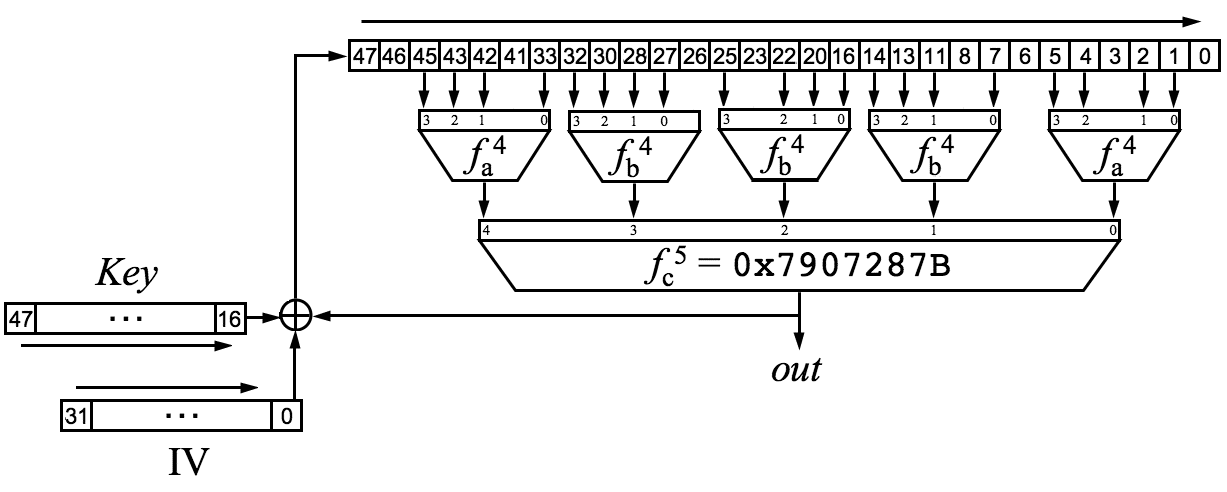
\includegraphics[width=5.5in]{./figures/hitag2-2.PNG}
	\caption{LFSR Setup Phase \cite{hitag2-figure}}	
	\label{fig:hitag2-2}
\end{figure}

\noindent \textit{\textbf{Output function.}} The output function consists of two levels of multiplexors. The multiplexors have fixed data bits, whereas the address bits are chosen either from the LFSR or from other multiplexors. In the first level, 20 bits from the LFSR are used as address bits to five four-bit multiplexors, giving a total of five bits of output (one from each multiplexor). These five bits are then used as address bits to the single five-bit multiplexor in the second level. The output bit of this multiplexor gives the stream cipher's output bit, constituting the keystream. In all, six instances of multiplexors cover the two levels of the output function.

\begin{table}[ht!]
\begin{center}
\small{
\begin{tabular}{|p{2.2cm}|l|p{2cm}|p{2.8cm}|p{1.5cm}|}
\hline 
\textbf{Multiplexor instance}	& \textbf{Function}		& \textbf{Data bits}	& \textbf{Address bits (input)}		& \textbf{Output bit}\\ \hline \hline
\multicolumn{5}{|c|}{Level 1 Multiplexors}\\ \hline \hline
MUX 1 			&	$f_a^4$			& 0x2C79			& 1, 2, 4, 5							& $o_1$\\
MUX 2 			&	$f_b^4$			& 0x6671			& 7, 11, 13, 14						& $o_2$\\
MUX 3 			&	$f_b^4$			& 0x6671			& 16, 20, 22, 25					& $o_3$\\
MUX 4 			&	$f_b^4$			& 0x6671			& 27, 28, 30, 32					& $o_4$\\
MUX 5 			&	$f_a^4$			& 0x2C79			& 33, 42, 43, 45					& $o_5$\\ \hline \hline
\multicolumn{5}{|c|}{Level 2 Multiplexor}\\ \hline \hline
MUX 6 			&	$f_c^5$			& 0x7907287B	& $o_1$, $o_2$, $o_3$, $o_4$, $o_5$		& $k_i$\\ \hline
\end{tabular}}
\end{center}
\caption{Multiplexors making the output function in HiTag2}
\label{tab:muxs}
\end{table}

Three different multiplexor functions are used to realize these six instances, and these are called $f_a^4$, $f_b^4$ and $f_c^5$. While $f_a^4$ and $f_b^4$ take in four bits for addressing the output, $f_c^5$ takes in five bits. The multiplexors $f_a^4$ and $f_b^4$ are used in the first level, where as $f_c^5$ is used in the second level. These six instances are described in the table \ref{tab:muxs}. In the table, the input bits for the first level of multiplexors are indicated by the index of their position in the LFSR.

It is important to note that the update function of the LFSR is not used in both the initialization and setup phases of the cipher. This function is used during the keystream generation as discussed next.\\

%The source code for the initialization and setup of the LFSR is shown below in the listing. Here, the function \emph{hitag2\_output} stands for the output function, which we have just described.\\

% NEEDED - explain a little about the implementation before the code snippet. 

%\lstinputlisting[frame=tb, caption={HiTag2 initialization code snippet}]{./code-snippets/hitag2_init.c}

\noindent \textit{\textbf{3. Keystream Generation.}} The output from the function $f_c^5$ constitutes the keystream. In addition, the LFSR state is changed in every clock cycle through the update function. The internal state is updated linearly, in the following fashion: the leftmost bit of the LFSR is replaced with the \textit{xor} of taps of the LFSR (which are bits 0, 2, 3, 6, 7, 8, 16, 22, 23, 26, 30, 41, 42, 43, 46 and 47). The remaining bits are shifted rightwards to adjacent positions. Once the internal state is changed, the output bit gets recomputed, generating the next bit of the keystream. This is shown in figure \ref{fig:hitag2-3}. 
%Following is the code snippet for the function implementing one round of the HiTag2 (\emph{hitag2\_round}), by first updating the state and then calling the output function (\emph{hitag2\_output}).\\

%\lstinputlisting[frame=tb, caption={HiTag2 keystream generation code snippet}]{./code-snippets/hitag2_round.c}

\begin{figure}[ht!]
	\centering
		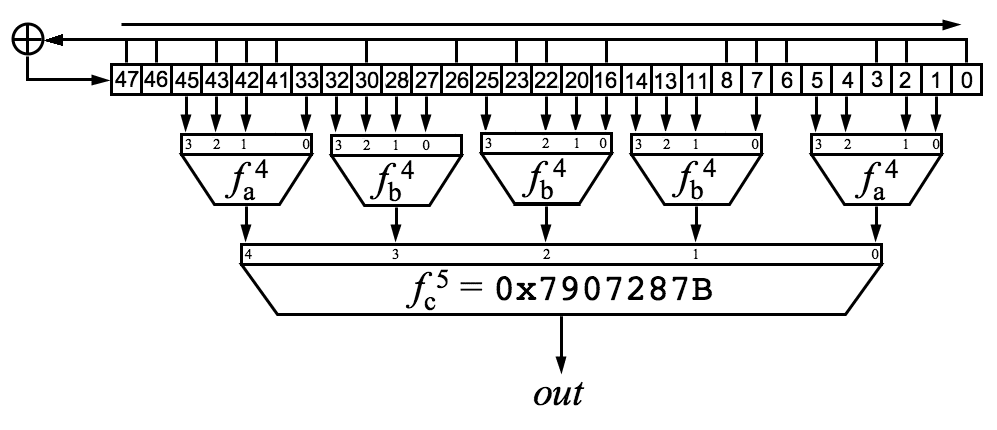
\includegraphics[width=4.3in]{./figures/hitag2-3.PNG}
	\caption{Keystream Generation \cite{hitag2-figure}}	
	\label{fig:hitag2-3}
\end{figure}

This completes a basic description of the cipher. 

A security critical aspect to consider here is the period of the HiTag2 LFSR. It is very important to note that the period of the LFSR is different from the period of the keystream (or period of the cipher). If the states of the LFSR repeat, then the keystream also repeats. But, the period of the keystream could be less than the period of the LFSR, as the output function is non-linear \cite{erik-discussions}. 

It is possible to check the period of the LFSR and ascertain if HiTag2 LFSR gives the maximal period of $(2^{48} - 1)$ or not. From previous discussion, the polynomial representation of the LFSR should represent an irreducible polynomial, if maximal period is to be achieved. We made an attempt to investigate this for HiTag2, but realized that huge computational time is required. In order to check if the HiTag2 polynomial is irreducible, all the factors of the polynomial need to be checked. This takes time of the order of $2^{48}$, which would take days to complete on a dedicated personal computer.

We encoded the polynomial in Matlab, as shown in appendix \ref{app:appendixA}. The program was run for a day without any decisive output. If the polynomial could be factorized by a small polynomial, the program would have shown the result and terminated; but this did not happen. Hence, we conclude that there are no small factors in the HiTag2 LFSR polynomial. On a more positive note, we believe that the polynomial is maximal, and we continue the rest of the thesis under this particular assumption.
\chapter{Time-memory tradeoff}

\paragraph{Summary}


\section{Time-memory tradeoff attack}

\textit{\textbf{Brute force attack.}} A brute force attack on a block cipher would be to try out all the possible keys which could be used to encrypt certain known (or chosen) or unknown plaintext. The key which decrypts the ciphertext to give the known plaintext or most sensible plaintext (if it is unknown) is then the original key. Though very simple in theory, brute force attacks require a very long time to break ciphers in practice. There is no storage required during this attack, but the time required to break the cipher is very long. Though modern computers have advanced tremendously in their computational speed over the last some years, design of new ciphers have incorporated longer key sizes to protect against brute force attacks, making brute forcing even more impractical.

For example, in order to break a 32 bit key, we would need to carry out $2^{32}$ decryptions on available ciphertext. Using a 2GHz processor (which is quite common for personal use), we can run $2^{31}$ clock cycles in one second (as 1 giga is $2^{30}$). Since one encryption would take a fixed number of clock cycles, say a modest $2^3$ cycles, by simple calculation, we can have a brute force attack on the cipher in $2^4$ seconds, or 16 seconds. As can be seen, this is a dismally weak key size. For a key size of 48 bits, the brute-force would take $2^{20}$ seconds which is 1048576 seconds, or just more than 12 days. In modern ciphers, the key sizes starting from 128 bits in length are considered safe. AES uses a minimum key size of 128 bits, which can be extended to use 256 bits. So, just to give a feeling of the security of a 128 bit cipher, it would take an order of $10^{30}$ years to brute force the key.\\

\textit{\textbf{Precomputed ciphertext attack.}} Brute-force attacks are just one side of the coin. The other way of breaking a cipher in a known (or chosen) plaintext attack is to precompute ciphertexts corresponding to all the possible keys and to store the (key, ciphertext) pair in a table in memory. During the attack, the attacker just needs to do a table lookup for the available ciphertext to find the corresponding key. Again, the concept is quite straightforward theoretically, but it also faces the same problem as brute-force attacks, but from a different perspective. A table lookup takes constant time (if efficient hash tables are implemented), so practically the attack time is very less. But, the amount of precomputed data is tremendous and the attacker would need very large amount of memory to save this data for the attack phase. 

Let us take the weaker case of a 32 bit key, which is far from use in today's ciphers. For each of $2^{32}$ possible keys, we need to store 32 bits of key and 32 bits of ciphertext (assuming the plaintext is 32 bits, which could very well be more). This amounts to 64 bits or 8 bytes of data for every possible key. $2^{32}$ such entries would require $2^{32}$ * 8 bytes which is 32 gigabytes. For a random access memory, 32 GB is a high requirement. For higher key sizes, this requirement gets more towards impossible.\\

\textit{\textbf{In between time and memory.}} The technique of time-memory tradeoff is a way between the above two extreme and practically difficult ideas. TMTO solves our problem by using memory in order to reduce the time taken for attack, bringing the requirements for time and memory within  practical domains. As a result, with considerable precomputation, the attack time can be reduced and so are the computational resources required.

Before we go into more details of the working of time-memory tradeoff attacks on ciphers, we would take a simple example of a general application of such tradeoffs. The example has been taken from \cite{stamp2003out}. \\

\textit{\textbf{Simple example.}} Consider the problem of finding the number of \textbf{1}'s in the binary expansion of a non-negative integer $x$ (which takes $4$ bytes). The simplest algorithm to solve this problem would for 32 operations, pick the value of the least significant bit, add it to a global \textit{sum} and shift the integer rightwards by one bit. The \textit{sum} would then be the desired result. The pseudo-code for such an algorithm is shown below.

\begin{verbatim}
// ones_count(x)
sum = 0
for i = 0 to len(x) - 1
    sum = sum + (x >> i) & 1
next i
return sum
\end{verbatim}

Here, $>>$ denotes the right shift operation and \& denotes bitwise binary \emph{and} operation. The algorithm performs 32 operations (based on the length of the integer) and has nearly no memory requirement. The other approach to solve this problem would be to store the required \emph{sum} for each of the possible $2^{32}$ integers in memory. This way, just one memory lookup is required to find the result for $x$. While in this case, we need to have a memory of the order of $2^{32}$. 

One middle way between both these approaches would be to store the \textit{sum} for all possible 8 bit numbers, rather than doing it for all 32 bit numbers. Then the memory required would be of the order of $2^{8}$. Then, we break the 32 bit integer into four bytes, and add the stored \textit{sum} for each of the four bytes, by looking up in the table. If $y_1$, $y_2$, $y_3$ and $y_4$ are the four bytes, such that

\begin{flushleft}
$y_4$ = ($x$ $\&$ $0$xFF)\\
$y_3$ = ($(x >> 8)$ $\&$ $0$xFF)\\ 
$y_2$ = ($(x >> 16)$ $\&$ $0$xFF)\\ 
$y_1$ = ($(x >> 24)$ $\&$ $0$xFF)\\
\end{flushleft}

and if p is the array which stores the \textit{sum} for all possible bytes, then the desired \textit{sum} for $x$ can simply be calculated by

\begin{center}
\large{$sum = p[y_1] + p[y_2] + p[y_3] + p[y_4]$}\\
\end{center}

The number of operations in this case is 4, as there are four lookups made to the precomputed array $p$. This is just one way of realizing a middle way between the parameters of time and memory. If the algorithm stores 4 bit values, with their corresponding \textit{sum}, then the number of operations would be 8. Hence a optimal combination of memory and time can be chosen based on the resources at hand and the application. 

% IMP: do you need to show the table here for different combinations of time and memory? %


\section{Background}
\subsection{Birthday paradox}
\label{sec:bday-paradox}

\textit{\textbf{General birthday paradox.}} Birthday paradox (or birthday problem or surprise, as it is also called), refers to the fact that in a room of 23 people, two people have the same date of birth with a probability greater than one-half. While there are 365 different possible birthdays in a year (excluding the leap year), the birthday paradox looks surprising and non-intuituve at the first glance. But, the figure has been derived from probability theory and is proved. 
% IMP: need a reference here %

A generalized definition of the birthday paradox for can be formulated as follows: given $n$ random integers where each could have $m$ different possible values, the probability that two of them would have the same value is given by the following equation \cite{menezes}.

\begin{center}
\large{$P(m,n)$ $\approx$ $1 - e^{-{n^2}/{2m}}$}
\end{center}

If we replace $m$ by 365, and $n$ by 23 in the above equation, then it can be checked that $P(365,23)$ $\approx$ $0.507$. In addition, $P(365,n)$ rapidly increases as $n$ increases, and the chances of two people having the same birthday becomes nearly $99 \%$ for $n$ = 57. If $m$ is considered to be very large, such that $m \rightarrow \infty$, then the above equation can be reduced, giving us the following condition for chances of nearly $100 \%$. 

\begin{center}
\large{$n$ = $\sqrt{\frac{\pi}{2} \times m}$}
\end{center}

The general birthday paradox is used in cryptography in determining collisions in hash functions. Consider a hash function $H$ with $h$ bits of output. The total number of different outputs the function could produce is $2^{h}$. A collision is said to occur when the hash function produces the same output for two different inputs, i.e. $H(x_1)$ = $H(x_2)$ when $x_1$ $\neq$ $x_2$. Then, according to the birthday paradox, the chances that a collision would occur are close to $100 \%$ after the hash function has produced outputs for $2^{h/2}$ random inputs (if we have $m = 2^h$ and we ignore the factor of $\frac{\pi}{2}$).\\

\textit{\textbf{Variant of the birthday paradox.}} A variant of the birthday paradox (\cite{GeneralizedAttack}) is especially more interesting to us, since it is directly used in TMTO attacks. If we consider two groups of people now instead of just one, then just 17 people are required to be present in each group, so that two people, one from each group, share the same birthday.  

We can generalize the above situation in the following way. We have two groups of random elements each having different number elements, say $n_1$ and $n_2$. The elements are non-negative integers, with both the groups having the same range $m$ for all the integers. According to \cite{menezes}, the probability of at least one coincidence in such a case is given by,
\begin{center}
\large{$P(m, n_1, n_2) = 1 -(1 -\frac{n_2}{m})^{n_1}$}
\end{center}

For the condition that $m \rightarrow \infty$, the above relation is reduced to,
\begin{center}
\large{$P(m, n_1, n_2)$ $\approx$ $1 - e^{-{n_{1} n_{2}}/{m}}$}
\end{center}

For there to be at least one coincidence, the probability must be $1$. Replacing $P(m, n_1, n_2)$ by $1$ and taking the limit $m \rightarrow \infty$, we get the following condition.
\begin{center}
\large{$n_1 \times n_2$ = $\frac{\pi}{4} \times m$ (or)\\}
\large{$n_1 \times n_2 \geq m$}
\end{center}

The last equation above is the birthday paradox we would be using the analysis of most of the TMTO attacks on HiTag2.

% Add the case of handbook statement, with or without replacements?
% also briefly how this paradox would be applied to the TMTO?

% -------------
% what the simple birthday paradox is %

% generalize it in terms of n %

% introduce birthday attack, define scenario (then take hash as example) %

% what is the variant of birthday paradox %

% meet in the middle attack on DES by diffie hellman %
% a TMTO attack would always use variant of birthday attack %

% Question - How can the variant of the birthday problem be derived from the birthday problem?
% Question - Probability of one-half on 23, or is it one? root(pi * m / 2)
% Question - Is meet in the middle attack a TMTO attack? (I think NO!)
% --------------

\subsection{Hash tables}
\label{sec:hash-tables}

Hash tables are used during the precomputation phase as a data structure to store the (prefix, state) pairs in memory. The advantage that hash tables offer is in terms of the search time. The search time provided by hash tables in the best case and the average case is close to $O(1)$, while the worst case search time is $O(n)$ occuring with very less probability. A very important role is played by the hash function chosen for the table. 

The basic data structure for hash tables consists of a pair of data elements, one for holding the \emph{value} to be stored, and the other which acts as a unique identifier for that value, called the \emph{key}. The hast table is basically an array of such (key, value) pairs. Typically in a normal array, pairs would be stored starting from the initial index of the array, with the index increasing with every pair. In a hash table, the pairs are not stored consecutively, but in an order which would make searching them more efficient at a later stage. The index at which a particular pair is stored depends on the key and the hash function. A hash of the key is calculated, and if required, reduced to the domain of the indices. The pair is stored at that index. 

While retrieving a value, the corresponding key is provided and hash of the key is calculated, giving the index of the pair. The index is used to retrieve the value from the array, which is a constant time operation. So, in the ideal scenario, a hash table can provide a constant time search algorithm. But due to the problem of collision, the search time increases by a certain factor. Collision occurs, if the same hash value (thus the same index) is computed for two different keys. In such a case, two different (key, value) pairs would contend to be stored at the same index, thus colliding.

Several proposals have been suggested to avoid the problem of collision. The most popular among them are linear probing and separate chaining. We discuss separate chaining here, since we have implemented this scheme for the two attacks in this section. The basic idea behind separate chaining is that if there is a collision at a particular index, a separate chain holding all the pairs for that index be created. In addition, a reference to the chain must be stored at that index in the array. During retrieval, the index is computed and the reference to the chain is taken from that index. At the reference location, the required value is retrieved by searching through the entire chain. 

The implementation of the hash table is done by Christopher Clark and has been taken from the web source \cite{hash-table-impl}, with due acknowledgement. 


\section{BG attack}
\label{sec:bg-attack}
Time-memory tradeoff attacks on stream ciphers are relatively new than those on block ciphers. The first TMTO attack which was conceptualized on the block cipher DES, was published by Hellman in 1980 \cite{hellman1980ctm}. In contrast, the first and the simplest TMTO attack on stream ciphers was published by Babbage \cite{babbage} and Golic \cite{golic}, independent of each other in 1995 and 1997 respectively. We would call this attack on stream ciphers as the BG attack. We explain the original BG attack and a variant of it in the sections \ref{sec:bg-r} and \ref{sec:bg-nr}.

\subsection{BG attack with random precomputation}
\label{sec:bg-r}

As discussed in section \ref{sec:psrg}, PRSG generates a long keystream using a short secret key, to which the bits of the plaintext are \emph{xor}'ed giving the ciphertext bits. In this way, a stream cipher is produced. A simple model of the PRSG taken from \cite{babbage} is shown in figure \ref{fig:psrg-model}. The initial state of the PRSG is $S_0$, which is derived using the secret key and other initialization parameters. The consequent states are indicated by $S_i$. The right arrow represents the update function while the downward arrow represents the output function. We assume that the PRSG incorporates an LFSR having the maximal period of $2^{n} - 1$.

\begin{figure}[h]
	\centering
	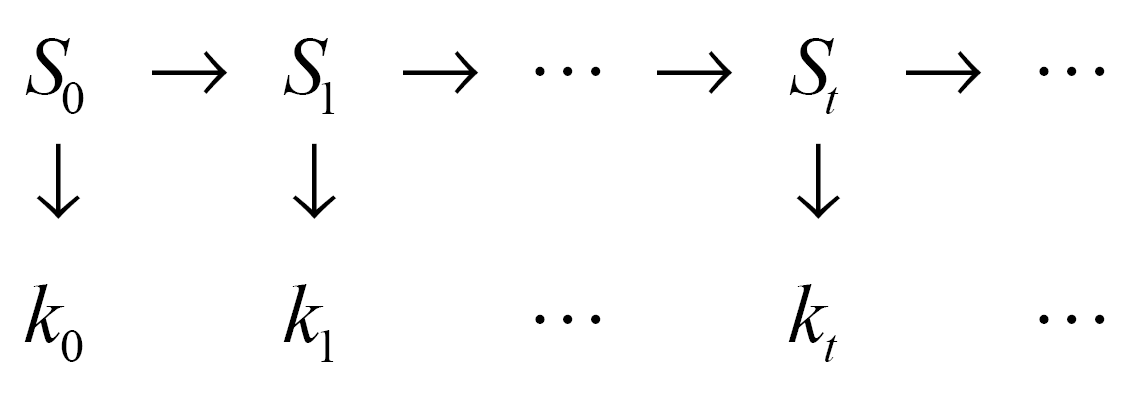
\includegraphics[width=3in]{./figures/prsgmodel.png}
	\caption{Model of pseudo-random sequence generator (PRSG)}	
	\label{fig:psrg-model}
\end{figure}

The keystream bits are represented by $k_0$, $k_1$ $\ldots$, $k_{m-1}$. The goal of the attacker is to find at least one internal state which occurs while the keystream is generated. The attacker could then move the PRSG forward to generate more keystream, in case the keystream is limited. The found internal state could also be used to run the PRSG backwards and find the initial state. From the initial state, finding the key is not a difficult task if the cipher algorithm and initialization parameters are known.\\

\textit{\textbf{Prefix of the output sequence of states.}} If the current state of the PRSG is $S_r$, then an infinite output sequence can be generated by clocking the PRSG from that state. The first $p$ bits of this output sequence is called the prefix of state $S_r$ and would be represented by the bits $k_r$, $k_{r+1}$ $\ldots$, $k_{r+p-1}$. Each of the $2^{n} - 1$ possible states of the PRSG would generate such an output sequence. The prefix of these sequences are usually unique to that particular state if $p$ is greater than or equal to $n$ \cite{biryukov2000rtc}. If the size of the prefix is less than $n$, then there would be many states which could possibly generate this prefix. For example, if the size of the state is 48 bits and we consider prefixes of size 32 bits, then the total number of states which generate this prefix is about $2^{48} \times 2^{-32}$ = $2^{16}$. If the size of the prefixes is increased to 48 bits which is also the size of the state, then there is usually just one state generating the prefix. By increasing the prefix length, the probability that the prefix is unique to the state increases. An advantage of this property is taken in the BG attack.\\

\textit{\textbf{The attack.}} We have two phases in the attack just as in any TMTO attack: the precomputation phase and the attack phase. During precomputation, the attacker randomly selects $n_1$ states out of the $2^n - 1$ possible PRSG states. For each of these states, the prefix of size $p$ = $n$ is computed, and the (prefix, state) pair stored in memory. The data structure that is used for storing the pairs is a hash table, introduced in section \ref{sec:hash-tables}.

During the attack phase, the attacker is assumed to know some part of the initial keystream. In practice, the attacker would know the ciphertext bits. And assuming that the attacker knows the plaintext bits by some means (a known plantext attack), the keystream is simply calculated in the following manner, $k_i$ = $p_i \oplus c_i$, as also mentioned in chapter \ref{chapter:intro}. The attacker then selects overlapping subsequences of size $p$ from the keystream. The first subsequence would be $k_0$, $k_1$ $\ldots$, $k_{p-1}$, the second subsequence would be $k_1$, $k_2$ $\ldots$, $k_{p}$ and so on. The attacker then matches each of these subsequences with the prefix's stored in the hash table. If there is a match, the current state is retreived from the matched (prefix, state) pair.\\

\textit{\textbf{Parameters in the attack.}} Before we proceed to an analysis of the above attack, we introduce the notation of important parameters used to describe the BG attack. These parameters would help us in understanding where an ideal line be drawn between memory and time consumption during the precomputation and attack phases, so that the attack is feasible say for example on a personal computer. These parameters are introduced below. 

\begin{enumerate}
\item \emph{M}, represents the order of memory size required for precomputation.
\item \emph{P}, represents the order of time required for precomputation.
\item \emph{T}, represents the order of time required for the attack phase.
\item \emph{D}, represents the order of the amount of data (in bits) available during the attack phase (length of the keystream).
\end{enumerate}

\textit{\textbf{Tradeoff equation.}} Let us assume that we select $n_1$ states during the precomputation phase and during the attack phase the PRSG traverses through $n_2$ states before the first match is observed. $M$ is equal to $n_1$, since the size of the hashtable would depend on the number of states stored in it. Similarly, the time to prepare the hashtable is proportional to $n_1$, hence the order of this time, or $P$, is $n_1$. As a result, $M$ = $P$ = $n_1$.

Similarly, $T$ is the same as $n_2$. Also, for sufficient number of subsequences to be available, the keystream should have a length of at least $(n_2 + n - 1)$ bits. Hence, $D$ = $(n_2 + n - 1)$. In such a case, the attacker would have exactly $n_2$ subsequences of length $n$ each to cover the attack time of an order $n_2$.

This is a clear setting for applying the birthday paradox. In a set of $2^n$ states, $n_1$ are selected in precomputation and $n_2$ are selected during the attack. According to the variant of the birthday paradox, explained in section \ref{sec:bday-paradox}, we then have the following condition:

\begin{center}
\large{$n_1 \times n_2$ $\geq$ $2^n$}\\
\large{$M \times T$ $\geq$ $2^n$}\\
\end{center}

This is the condition that we required for a successful attack. Though this is probabilistic, we know that if the parameters of $M$ and $T$ are wisely chosen, the probability of a match becomes very high.

\subsection{BG attack with non-random precomputation}
\label{sec:bg-nr}

The precomputation in BG attack is done by randomly generating states of $n$ bits, and then computing their prefix. The other way of performing the precomputation is by selecting states through a deterministic algorithm. Consider that the internal state in a stream cipher runs through all $2^n - 1$ possible states, represented by a huge cycle of states as shown in figure \ref{}. If we select states at a fixed distance $d$ from each other during precomputation, we can be sure that there would be a match if the attack phase has a time order of $d$ \cite{erik-discussions}. This is the main idea behind non-random precomputation and is explained in detail in the further paragraphs. The HiTag2 cipher is well suited for this attack, since it's internal state runs through the longest possible cycle of size $2^n - 1$. The attack phase for this attack remains the same as in case of randomly selected precomputation states.\\

\textit{\textbf{Non-random precomputation phase.}} During the precomputation phase, the selection of states is not done at random. Only an initial state is selected at random for precomputation ($S_{initial}$), while the remaining states are derived using this state. The prefix for $S_{initial}$ is first computed and the (prefix, state) pair stored in the hash table. The next state is derived using a \emph{state transition function} (explained in detail later), which returns the state $d$ states ahead of the current state. The next state then is represented by $S_{initial+d}$. Similarly, the prefix for $S_{initial+d}$ is computed and the (prefix, state) pair stored in the hash table. The process is repeated, and consequently we have a set of states (and the corresponding prefix) in memory. These would be $S_{initial}$, $S_{initial+d}$, $S_{initial+2d}$ and so on. Until the complete circle of states is covered (after which the same states are repeated) we have unique (prefix, state) pairs. At the end of the precomputation phase, we would have a total of $2^n/d$ states in the hash table. The precomputation phase would take memory space of an order of $2^n/d$. It can be clearly seen that $M$ and $P$ would be the same in this case as well, and we have the relation $M$ = $P$ = $n_1$ = $2^n/d$.\\

\textit{\textbf{Attack phase.}} Let us assume that the initial state generating the available keystream is $S_{unknown}$ (as this state is unknown to the attacker). The attacker selects subsequences from the keystream and matches them with the prefixes stored in the memory. If the attacker gets $d$ subsequences from the keystream (which represent $d$ unknown states), a prefix in the memory is bound to get matched with a keystream subsequence. Hence, in the worst case, a traversal through $d$ states would be required during the attack phase, taking $d$ order of operations before a match in the memory. $T$ in this case would be $T$ = $n_2$ = $d$, while $D$ becomes $D$ = $(d + n - 1)$.\\

\textit{\textbf{Tradeoff equation.}} It can be clearly seen that the following relation holds,

\begin{center}
\large{$M \times T$ = $2^n$}\\
\end{center}

Using this equation, the tradeoff in memory and time can be achieved. It is interesting to compare this equation with the equation for BG attack with random states during precomputation. The latter was based on the birthday paradox, and hence the probability of finding a match is always close to \textbf{1}, but not exactly \textbf{1}. The greater the value of $M \times T$ is as compared to $2^n$, more is this probability closer to \textbf{1}.

In case non-random states are chosen during precomputation, the probability of a match is exactly \textbf{1}, provided the above tradeoff equation holds. This ofcourse assumes that $n$ bits of prefix uniquely identify the state generating it. But this is not the case always, as we shall see from our implementation results. In order to be sure that the prefix uniquely identifies a state, a greater length of prefix should be chosen.\\

\textit{\textbf{Matrix representation of state transition function.}} As mentioned above, the \emph{state transition function} is used in the precomputation phase for deriving a non-adjacent state from the current state. If we use the update function in order compute the state $d$ distance ahead, the function would be called $d$ times and thus take a total computation time of an order $d$. If this has to be repeated in order to cover the entire cycle of states, the computation time required would be of the order of $2^n$. Ofcourse, this is not feasible, otherwise we would very well launch a brute force attack on the internal state. A function is required which derives the $d$'th state in constant time, thus reducing the precomputation time order to $2^{n}/d$. We call such a function the state transition function, and its design is discussed here. 

An update function is used in deriving the adjacent state, which can be represented by a binary matrix $U$ \cite{trappe2005icc}. This matrix on multiplication with the matrix representing the current state gives the adjacent state matrix. If the current state of the LFSR is $S_{current}$, then the next state $S_{next}$ can be computed by the matrix multiplication shown below.

\begin{center}
\large{$U . S_{current}$ = $S_{next}$}\\
\end{center}

This is represented in the matrix notation as follows.

\begin{center}
\large{
$U.$
$\begin{bmatrix}
s_{n} \\
s_{n-1} \\
\vdots \\
s_{1} \\
s_{0}
\end{bmatrix}$ = 
$\begin{bmatrix}
s_{new} \\
s_{n} \\
\vdots \\
s_{2} \\
s_{1}
\end{bmatrix}$}
\end{center}

The topmost row of $U$ would represent the tap sequence by containing \textbf{1} at positions representing the tap bits, and \textbf{0} otherwise. It is so because this row is multiplied with the current state to give the new bit (the leftmost bit) of the LFSR. The remaining rows of $U$ are setup in such a way that the remaining bits of the LFSR are shifted one place rightwards. It must be noted that the indexing in the matrix is the same as that in the LFSR. Thus, the leftmost position in the any row of $U$ is for the \textbf{48}'th bit of the LFSR, and the rightmost position is for the \textbf{1}'st bit. In addition, in the state matrices $S_{current}$ and $S_{next}$, the topmost position is for the \textbf{48}'th bit of the LFSR, and the bottommost position is for the \textbf{1}'st bit. The matrix $U$ for HiTag2 is shown in figure \ref{fig:hitag2-transition-matrix} as an example.

\begin{figure}[h!]
	\centering
	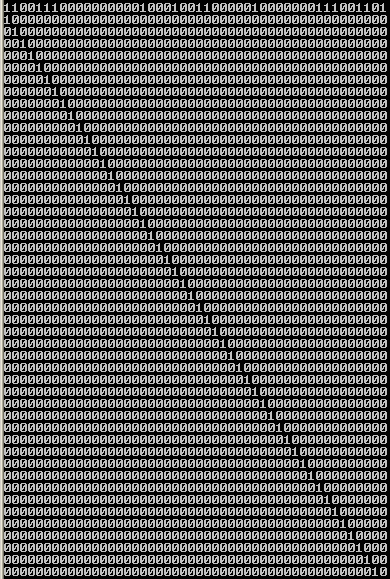
\includegraphics[width=3.5in]{./figures/hitag2-transition-matrix.png}
	\caption{Update function matrix $U$ for HiTag2}	
	\label{fig:hitag2-transition-matrix}
\end{figure}

Matrix multiplication for binary matrices is to perform a bitwise boolean \emph{and} operation (denoted by \&) and then \emph{xor} the resulting bits. In notation, if we have two rows $r_1$ and $r_2$ of size $n$ for multiplication, then we have the following,

\begin{center}
\large{$r_1$ = $r_{11} r_{12} \ldots r_{1n}$}\\
\large{$r_2$ = $r_{21} r_{22} \ldots r_{2n}$}\\
\large{$r_1 \times r_2$ = $(r_{11} \& r_{21}) \oplus (r_{12} \& r_{22}) \oplus \ldots \oplus (r_{1n} \& r_{2n})$}
\end{center}

To compute the state occuring $d$ states after the current state, we perform the above matrix multiplication $d$ times, as follows,

\begin{center}
\large{$S_{current + d}$ = $\underbrace{U . U . U \dots U}_{d} . S_{current}$}, or\\
\large{$S_{current + d}$ = $U^d . S_{current}$}\\
\end{center}

From \cite{erik-discussions}, there is an efficient solution for computing the states. Instead of performing matrix multiplication of $U$ $d$ times, a repeated square of the result can be performed. The square of $U$ is first computed giving $U^2$. This is squared to compute $U^4$, which is again squared to compute $U^8$, and so on. If $\log_2{d}$ is an integer, then the squaring is repeated for $\log_2{d}$ number of times, as shown below.

\begin{center}
\large{$S_{current + d}$ = $\underbrace{(((U^2)^2) \dotsc )^2}_{\log_2{d}} . S_{current}$}\\
\end{center}
\label{eq:state-trans}

As can be seen, computing each state would take $\log_2{d}$ multiplications, and thus the entire precomputation phase would take $d \times \log_2{d}$ matrix multiplications. This is much effecient than the previous complexity of $2^n$. The above equation shall then be used in the precomputation phase of this attack to compute the (prefix, state) pairs.

\subsection{Implementation details}
% implementation results %
% TMD calculations, specially data requirement for the attack %

Both the versions of the BG attack differ only in the way the precomputation phase proceeds. In the implementation, we have identified these different ways by using a variable named \emph{memory\_setup} which either has the value RANDOM\_MEMORY or NON\_RANDOM\_MEMORY. Depending on this parameter, the appropriate functions are called.\\

\textit{\textbf{Using random function.}}
In order to randomly select states for precomputation, we need a random function. The $rand()$ function provided by C library is not a cryptographically strong function. Initially, the rand() function was used. Based on its short period, the desired number of different states could not be generated. 

\textit{\textbf{Computing state transition function.}}


\textit{\textbf{Preparing keystream.}}


\textit{\textbf{Setup hashtable.}}


\textit{\textbf{Running attack.}}




\section{TMTO attack with limited keystream}

In the previous attack, there is an assumption on the length of keystream available to the attacker. The minimum number of operations required to be performed during the attack phase (or $T$) in order to find a match determines the required length of keystream. Considering the use of HiTag2 in car keys, it is certain that long keystream would not be available. Rather several short length keystream (for each transaction between the car and car key) would be available over some span of time. As explained in section \ref{sec:hitag2}, 32 bits of data is exchanged between the car and the car key in the beginning of every run of the protocol. The complete protocol is not known to us, but it is just known that these 32 bits are sent across from the car controller to the key \cite{email-ruptor}. Along with the 32 bits, an IV is also sent. The car key then initializes the HiTag2 cipher using the shared secret key, the IV and its serial ID, and matches the computed output of the cipher to the received 32 bits. These 32 bits of data, known as the \emph{authenticator tag}, perform the function of authenticating the car to the car key. After authentication is successful, subsequent messages if any, are encrypted using the subsequent keystream.

Thus for this particular attack, we assume the availability of authenticator tags to the attacker. Also, we ignore any knowledge of further keystream. Hence the goal is to find the secret key just by using several authenticator tags. The difference between the tags lies in different initial state arising due to a different IV sent by the car. The secret key shared between the car and the car key is the same, and so would be the serial ID of the car key.

\subsection{TMTO tags attack}

The TMTO tags attack consists of the two TMTO phases: precomputation and attack. The precomputation phase involves selecting $M$ different initial states, computing their tags and storing the (tag, initial state) pair in a hashtable. The time for preparing the precomputation phase is of the order of $M$, since the complexity lies in the number of tags chosen for the phase. Hence, we also have $P$ = $M$.

During the attack phase, tags are randomly generated along with their corresponding IV's (to simulate the tags collected by an attacker). These tags are then matched with the tags in the hashtable. For every tag match in the hashtable, the initial state is referred and the key used to initialize the cipher to that state is computed. Since each tag can be generated by approximately $2^n/2^{32}$ states, we cannot be sure that the initial state found is the one we are looking for. Hence, we continue with the matching of further tags until we find that the same key is recovered more than once. Then we can be more sure that it is the correct secret key.\\

\textit{\textbf{Tradeoff equation.}} Determining the tradeoff equation in the tags attack is discussed here. Getting to the equation is not as straightforward as in the previous attack cases, but the results are strikingly similar.

Let us first consider the probability of finding a match in the hashtable. If the order of the memory required during precomputation is $M$, then we have $M$ different states and corresponding tags. It cannot be guaranteed that all the tags would be different, since a tag would have more than one possible geenrating states. In the best case, we assume that all the $M$ states generate $M$ different tags. Then, in this case, the probability of getting a tag matched in the hashtable is given by $M/2^{32}$, considering 32 bit tags. We write this probability as $P_1$, such that

\begin{center}
\large{$P_1$ = $M/2^{32}$}
\end{center}

Again, this is the best case probability and the actual probability would be less, since tags would be repeated in the hashtable. Next, we need to determine the probability that a match yields the correct initial state and thus the correct key. This can be determined in the following way: the total number of states is $2^n$ and the total number of tags is $2^{32}$. Then, the probability that the matched tag be representing the correct internal state is $2^{32}/2^n$. This probablity is represented by $P_2$ such that

\begin{center}
\large{$P_2$ = $2^{32}/2^n$}
\end{center}

The overall probability of finding the correct state is given by $P$, such that

\begin{center}
\large{$P$ = $P_1 \times P_2$}\\
\large{$P$ = $M/2^{n}$}\\
\end{center}

This is the probability of the correct key being found when we have one tag. Hence, for the probability to be \emph{1}, the runtime of the attack phase must be of an order of $2^{n}/M$ altleast, so that we have $2^{n}/M$ tags. Hence, we can say that

\begin{center}
\large{$T \geq 2^{n}/M$}\\
\large{$M \times T \geq 2^{n}$}
\end{center}

In practice, the product of $M$ and $T$ must be larger than $2^n$, since we considered the best case probability while calculating $P_1$. Practically, $P_1$ would be less than its value in the above equation, which would lead to a lower $P$. With lower $P$, $T$ would have to increased if we want to find the correct state. The equation for $P$ just gives us an approximate value of $M$ and $T$, and it is quite possible that the attack is successful for higher values of the two parameters.
\chapter{Time-memory-data tradeoff using Hellman tables}
\label{chapter:tmdto-hellman}

\indent \textbf{\textit{Summary.}} In sections \ref{sec:bg-keystream-attack} and \ref{sec:bg-tags-attack}, we described two TMTO attacks designed particularly for stream ciphers. They take into account two set of states: one set computed during the precomputation phase, and the other set containing states traversed during the attack phase. A common state is desired to occur between these two sets, and the parameters of the attack are chosen in order to have high chances of this occurence.

The attacks we describe in this and the next chapter are different from these two attacks. These attacks were originally designed for block ciphers. By making certain changes to the attack schemes, tradeoff attacks for stream ciphers are proposed. The Hellman attack is the one we consider in this chapter. First, the original attack for block ciphers is described. Then using this, Biryukov and Shamir attack is described for stream ciphers with their tradeoff equation. Further, we propose a general tradeoff equation for the attack and present results from the implementation using this general tradeoff.

\section{Hellman tables for block ciphers}

A block cipher is an encryption algorithm, which takes in a plaintext block of $n$ bits (called the block size) and a key of $k$ bits, and returns a ciphertext block of $n$ bits. Figure \ref{fig:block-cipher} illustrates a simple block cipher, with plaintext, ciphertext and key represented by $P$, $C$ and $K$ respectively. The encryption function is denoted by $E$ such that $C$ = $E_K(P)$ and implying encryption of $P$ under $K$.

\begin{figure}[ht!]
	\centering
		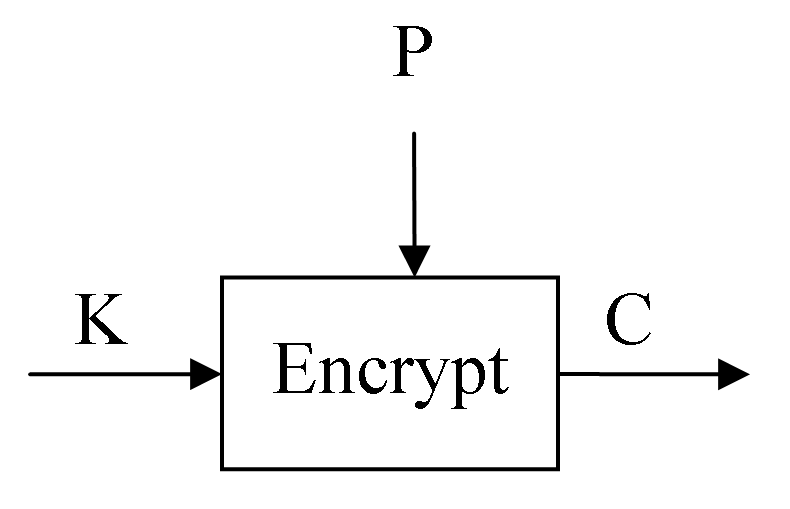
\includegraphics[width=2in]{./figures/block-cipher.PNG}
	\caption{A block cipher}	
	\label{fig:block-cipher}
\end{figure}

We first present the idea of the attack under certain ideal assumptions. Later we build upon this idea by considering the practical problems and their mitigation in a more practical attack.

\subsection{The ideal TMTO attack}
In the general scenario of an attack on block ciphers, the attacker has knowledge of a particular plaintext block $P$ and the corresponding ciphertext block $C$. The goal is to find $K$, using which the attacker can decipher ciphertext corresponding to unknown plaintext. For simplicity we assume the size of $K$ to be equal to the block size of $n$ bits. Then consider the following precomputation phase.\\

\noindent \textit{\textbf{Precomputation phase.}} An $n$ bit value is randomly selected using a uniform distribution (and denoted by $SP$ for a starting point). Using $SP$ as a key (denoted by $K_0$), encryption of $P$ is performed. The ciphertext obtained from this encryption is then used as the key (denoted by $K_1$) for the subsequent round of encryption of $P$. This procedure is iterated over a total of $t$ encryptions, yielding the key $K_t$ at the end. The key $K_t$ is called an end point, and is represented by $EP$. Moreover, the sequence of encryptions starting from $SP$ to $EP$ is called a \emph{chain} and is illustrated in the figure \ref{fig:block-cipher-single-chain}. Equations for the $t$ encryptions are also shown below. 

\begin{align*}
& & K_0 &= SP & & & &\\
1&. & K_1 &= E_{K_0}(P) & & & &\\
2&. & K_2 &= E_{K_1}(P) & & & &\\
& & &\vdots & & & &\\
(t-1)&. &K_{t-1} &= E_{K_{t-2}}(P) & & & &\\
(t)&. &K_{t} &= E_{K_{t-1}}(P) & & & &\\
& & EP &= K_{t} & & & &\\
\end{align*}

\begin{figure}[ht!]
	\centering
		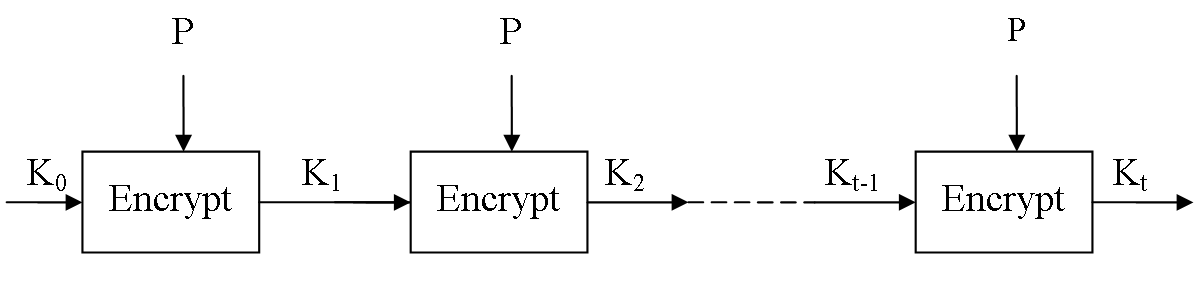
\includegraphics[width=5.5in]{./figures/block-cipher-single-chain.PNG}
	\caption{A chain of encryptions}	
	\label{fig:block-cipher-single-chain}
\end{figure}

During the precomputation phase, the goal is to cover the entire key space such that all possible keys exist in the table structure. A single chain covers a total of $t$ distinct keys. Though the chain contains a total of $(t+1)$ keys starting from $K_0$ to $K_{t}$, only the first $t$ keys are useful during the attack phase. This we shall explain later, and for the moment we note that only $t$ keys are represented in the chain.

An appropriate length $t$ of the chain is chosen so that no key repeats in the chain. Repetition is not desired since once a key reappears, subsequent keys would also repeat, adding no extra information to the chain. Hence, the size of the chain is restricted, and more than one chains are created instead. 

Lets say $m$ more such chains are needed to cover all possible keys. If we consider the ideal case in which each chain contains $k$ distinct keys, then we have $m$ = $2^n/t$. For each chain, we select a random starting point $SP_j$ and compute the end point $EP_j$, for $1 \leq j \leq m$, as shown in figure \ref{fig:single-chain}. Only the pairs $(SP_j,EP_j)$ are then stored in a hashtable, with $EP_j$ as the hashkey and $SP_j$ as the corresponding hashvalue. All the chains representing such a table structure are illustrated in the figure \ref{fig:naive-hellman-table}.

\begin{figure}[ht!]
	\centering
		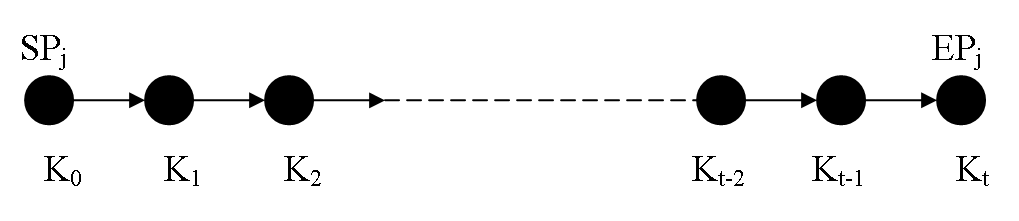
\includegraphics[width=4in]{./figures/single-chain.PNG}
	\caption{A single chain of encryptions represented by the pair $SP_j$ and $EP_j$}	
	\label{fig:single-chain}
\end{figure}

\begin{figure}[ht!]
	\centering
		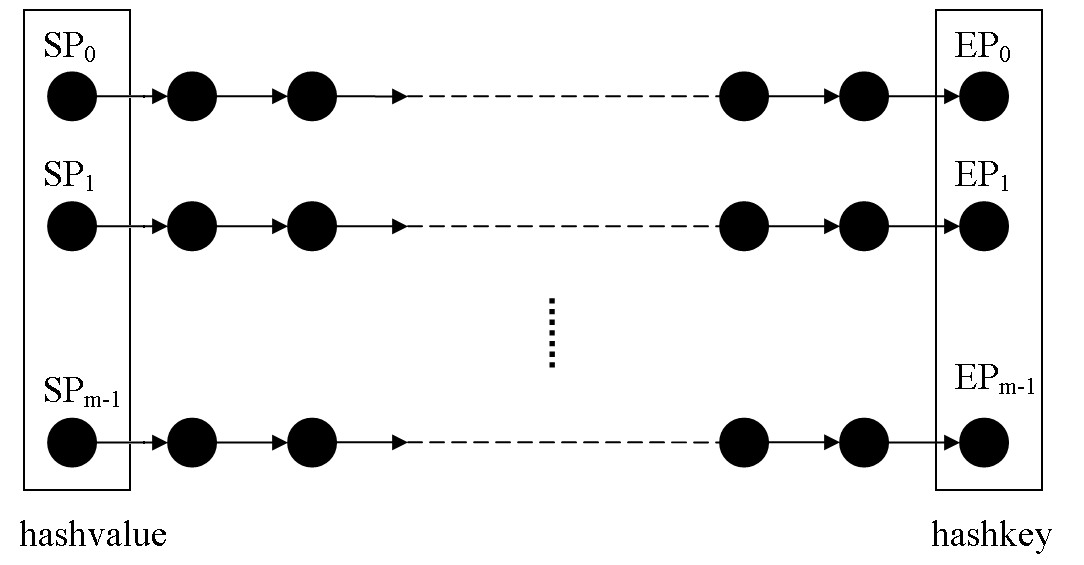
\includegraphics[width=4.5in]{./figures/naive-hellman-table.PNG}
	\caption{An ideal case Hellman table structure}	
	\label{fig:naive-hellman-table}
\end{figure}

We now compute $M$ and $P$ for the precomputation phase. The size of the memory required for storing all the chains would be of the order of $m$ as for each of the $m$ chains, a constant number of elements ($SP$ and $EP$) are stored. Thus we have $M$ = $m$. Also, as there are $mt$ encryptions performed in the entire table, the precomputation time is given by $P$ = $mt$.\\

\noindent \textit{\textbf{Attack phase.}} It is easy to see that if the required key $K$ exists among the first $t$ keys in any chain, the ciphertext $C$ would also exist. The possible locations of $K$ thus in every chain are from $K_{j,0}$ to $K_{j,t-1}$. The key $K_{j,t}$ is not considered to be a possible key since it is not used in the encryption of $P$. Or in other words, the ciphertext obtained from $K_{j,t}$ is not computed and thus not stored in the chain, hence it cannot be matched with the available ciphertext $C$. So, there are $t$ possible values for $K$ per chain. Looking at this from the perspective of $C$, there are also $t$ possible values of ciphertext in every chain that can match with $C$. These $t$ possible matches correspond to each of the $t$ possible keys, and range from $K_{j,1}$ to $K_{j,t}$.

The first possibility is that $C$ lies in $t$'th column of any one of the $m$ chains. This is true only if $C$ equals some $EP_j$ stored in the hashtable. In such a case $K_{j,t-1}$ is the key we are looking for. To find this key, we retrieve $SP_j$ corresponding to $EP_j$ from the hashtable and perform $(t-1)$ encryptions on $P$ using $SP_j$ as the key for first encryption followed by the ciphertext from one encryption as key for next encryption. After $(t-1)$ encryptions the desired key $K_{t-1}$ is obtained. 

If $C$ does not match any of the $EP_j$, the next possibility is that $C$ lies in the $(t-1)$'th column of some chain. If this is indeed the case, then $X$ = $E_{C}(P)$ must match with some $EP_j$. On a match, we know that the key $K_{j,t-2}$ is the required key. To find out $K_{j,t-2}$, we retrieve $SP_j$ correspondng to the matched $EP_j$ and perform $(t-2)$ encryptions. 

If none of the $EP_j$ matches with the evaluated $X$, we explore the possibility of $C$ lying in the remaining columns, one by one.

If $C$ exists in any chain, then the time taken to find $K$ is the same as the length of each chain. Assuming $C$ exists in the $r$'th column (such that  $2 \leq r \leq t$, then $X$ is computed by performing $(t-r)$ encryptions in the following way.

\begin{align*}
& & K_r &= C & & & &\\
1&. &K_{r+1} &= E_{K_r}(P)  & & & &\\
2&. &K_{r+2} &= E_{K_{r+1}}(P) & & & &\\
& & &\vdots & & & &\\
(t-r) &. &K_{r + (t-r)} &= E_{K_{r + (t-r-1)}}(P) & & & &\\
& & X &= K_{r + (t - r)} & & & &\\
\end{align*}

If $X$ matches an $EP_j$, then $(r-1)$ encryptions are performed to retrieve the key $K_{r-1}$. So in all, the number of encryptions performed is $(t-r) + (r-1)$ = $(t-1)$. Thus, the attack time is of the order of $t$ and our attack parameter $T$ = $t$.\\

\noindent \textit{\textbf{Problems with above approach.}} The approach described above is an ideal case, and some serious problems exist with it.

\begin{enumerate}

\item We have assumed that the length of $K$ is equal to the block size. This assumption does not hold for practical block ciphers, and thus we need to design a solution considering different key length and block size. Generally, the block size is larger than the key length. Thus a reduction function $R$ is required for the conversion of $n$ bits of $C$ to $k$ bits of $K$, where $n > k$. 

% some example reduction functions

During precomputation, the encryption function is replaced with the new function, which performs encryption and reduction to give the new key. This function is called the \emph{mapping function} (denoted by $f$), since it maps one key to another in the same keyspace. Such a mapping function is shown in figure \ref{fig:mapping-function}. 

\begin{figure}[ht!]
	\centering
		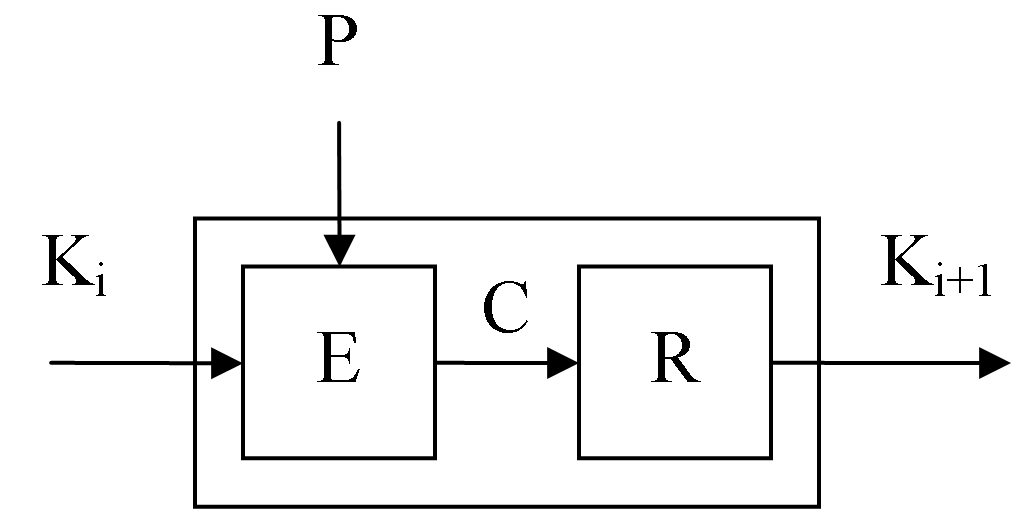
\includegraphics[width=3in]{./figures/mapping-function.PNG}
	\caption{Mapping function for block ciphers}	
	\label{fig:mapping-function}
\end{figure}

The function can also be represented in notation as follows, where $R$ stands for the reduction function.

\begin{center}
$K_{i+1}$ = $f(K_i)$ = $R(E_{K_i}(P))$\\
\end{center}

\item A much more serious problem in the ideal case is the assumption that all possible keys exist in the table structure and that no key is repeated. It is desired that all keys are covered, but practically this is hard to achieve. As more and more keys exist in the table, repetition of keys becomes frequent. The rate of repetitions grows exponentially after a certain number of keys making inclusion of new keys difficult in the table. This claim is can be proved using equation \ref{eq:bday-paradox2} of the birthday paradox.

Suppose we have $m$ chains with $t$ keys each so far in the table. A new chain is then added to the table. The total number of keys existing in the table are $mt$ while $t$ more keys are added through the new chain. We are interested in restricting $m$ and $t$ so that there is no common key between the $m$ chains and the new chain. According to the variant of the birthday paradox, the product of the sizes of these two sets should be less than or equal to the keyspace size, in order to have a high probability that no common key exists. Then, we have 

\begin{center}
$mt \times t \leq 2^k$\\
$mt^2 \leq 2^k$\\
\end{center}

If the $<$ condition is removed, then we have an upper bound on the value of $mt^2$ called the \emph{table stopping rule} and represented by the condition 
$mt^2 = 2^k$. 

In the ideal case described above, number of keys covered in the $m$ chains is $2^k$, which implies $mt = 2^k$. If we use this equation in estimating the value of $mt^2$, it can be seen that $mt^2$ is much greater than $2^k$. This is not allowed according to the table stopping rule, and thus lots of keys would repeat in our ideal table structure. Repetition of keys gives rise to the problems of \emph{collision and merge} during the precomputation phase and \emph{false alarms} during the attack phase. We explain these two problems below.
\end{enumerate}

\noindent \textit{\textbf{Collision and merge.}} Consider any two chains in the precomputation table structure. If there is a common key $K_c$ existing in both the chains, then the sequence of keys appearing after $K_c$ would be the same in both chains, as shown in figure \ref{fig:collision-merge}. There would be overlapping keys in the two chains resulting in wastage of precomputation time since they add no extra information to the chains. Such a situation is called collision.\\

\begin{figure}[ht!]
	\centering
		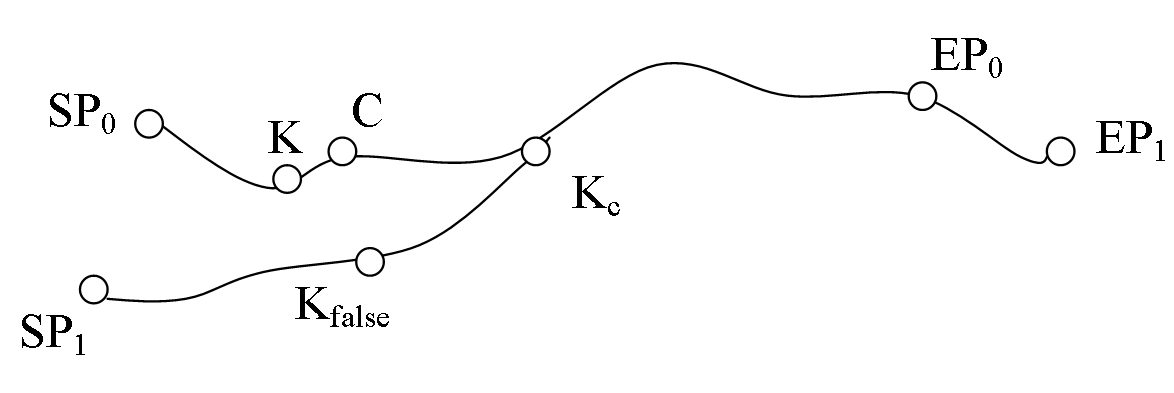
\includegraphics[width=4.5in]{./figures/collision-merge.PNG}
	\caption{Two chains which collide and consequently merge}	
	\label{fig:collision-merge}
\end{figure}

\noindent \textit{\textbf{False alarms.}} Colliding and merging chains during precomputation affect the attack phase as well. Consider the same example of the two chains colliding at $K_c$. Suppose that the required key $K$ appears in the first chain as shown in figure \ref{fig:collision-merge}. During the attack phase keys are computed starting from $C$ till one of the key matches an end point in the hashtable. 
In the example, a match would occur at $EP_0$ since $EP_0$ is one of the keys in the path from $C$ to $EP_1$ and $EP_0$ exists in the hashtable. The hashtable returns the starting point $SP_0$ for the match, and thus a key is derived from $SP_0$ ($K_{false}$). This key is different from the desired key $K$ since it lies in a different chain, as the two chains collide and merge. A false alarm is said to have occured here.

The occurence of false alarms can be easily checked and ignored. It is expected that the ciphertext obtained by encrypting $P$ under the derived key be the same as $C$. The ciphertext obtained using $K_{false}$ is not the same as $C$ as both the keys are different. This confirms that $K_{false}$ is not the right key. The only problem with false alarms is that they waste time during the attack phase and thus increase the attack time for finding the correct key.\\

\noindent \textit{\textbf{Solving the problem of collision.}} The inclusion of reduction function does not help in solving the problem of collision. Collisions still have the same effect if mapping function $f$ is used instead of encryption function $E$. But, if we use different reduction functions (hence, different mapping functions) for two colliding chains, the two chains do not merge and produce different keys from the colliding point $K_c$. Even though the ciphertext computed from the colliding key would be same, different reduction functions in the two chains ensure different keys, thus preventing merging of the chains. Such a scenario is shown in figure \ref{fig:collision-not-merge}. 

\begin{figure}[ht!]
	\centering
		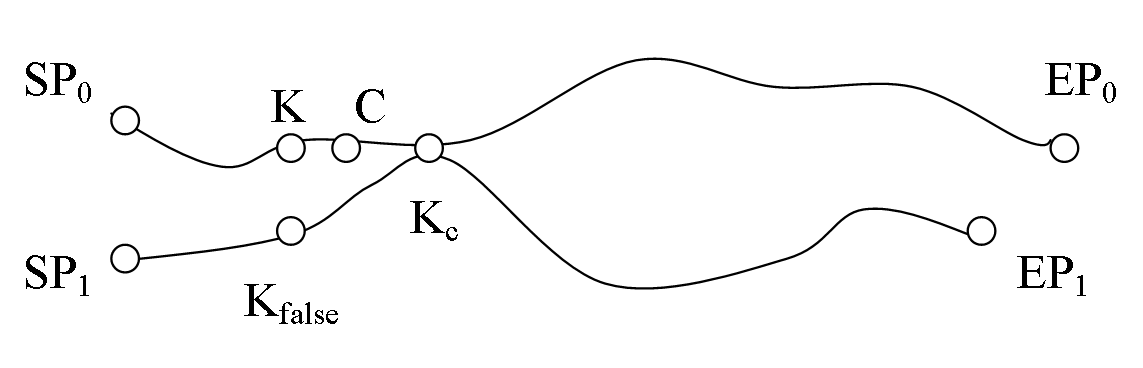
\includegraphics[width=4.5in]{./figures/collision-not-merge.PNG}
	\caption{Two chains which collide but do not merge}	
	\label{fig:collision-not-merge}
\end{figure}

As shown, the two chains terminate at different end points. As a result, when a match occurs during the attack phase, the correct end point is retrieved from the hashtable and consequently the correct key is obtained. 

But practically, using $m$ different mapping functions for building the table has problems. Stamp and Low quote in \cite{stamp2007acb} that having $m$ mapping functions makes storage of these functions resource intensive, and thus that it's not a good idea. An apparent and more serious problem though, with having $m$ mapping functions, is that the attack phase would run for a long time. During the attack phase, the given $C$ must be evaluated for all the different mapping functions because the attacker does not know the chain in which $C$ appears. The attack time in such a case becomes proportional to $mt$. 

In any case, the idea of having different mapping functions for each chain is not feasible. But, the use of mapping function provides a basis for a more practical table structure for block ciphers. 

\subsection{The practical TMTO attack}

Based on various ideas gathered from the previous section, the idea of Hellman tables \cite{hellman1980ctm} is presented here. The two important features of Hellman tables are the following,

\begin{enumerate}
\item There are multiple tables in the precomputation, as compared to the previously considered one big table. The total number of tables is denoted by $r$. Each table has a different mapping function, and thus collision occuring among chains belonging to different tables do not result in a merge.

\item In order to reduce the possibility of collisions occuring among chains within same tables, the size of each table is restricted in accordance with the \emph{table stopping rule}. Hence the relation $mt^2$ = $2^k$ must hold.
\end{enumerate}

We describe in detail the precomputation and attack phase for the TMTO attack using the Hellman tables.\\
% need some thing more here.

\noindent \textit{\textbf{Precomputation phase.}} First, $r$ different random reduction functions are chosen, say \mbox{$R_1$, $R_2$, \ldots ,$R_r$}. Using each of these functions, $r$ tables are created in the same way as described for the ideal case. Each of the $r$ tables consist of $m$ chains with $t$ keys and use mapping function $f_i$. Also, for each table, a different hashtable is created such that the starting and end points of the chains from that table are stored in the corresponding hashtable. Such a table structure is shown in figure \ref{fig:hellman-tables}, which is taken from \cite{oechslin:mfc}.

An important observation can be made from the figure: the number of computations in a chain is $(t-1)$, and not $t$ as we have been discussing. The same scene is observed in \cite{stamp2007acb} as well. With $(t-1)$ computations, $(t-1)$ keys exist in each chain. If $t$ is large as compared to 1, then $(t-1) \approx t$. Hence in these references, the number of keys in every chain is assumed to be $t$ for all analysis. On the other hand, we have assumed exactly $t$ keys per chain for the analysis and have also implemented the same.

\begin{figure}[ht!]
	\centering
		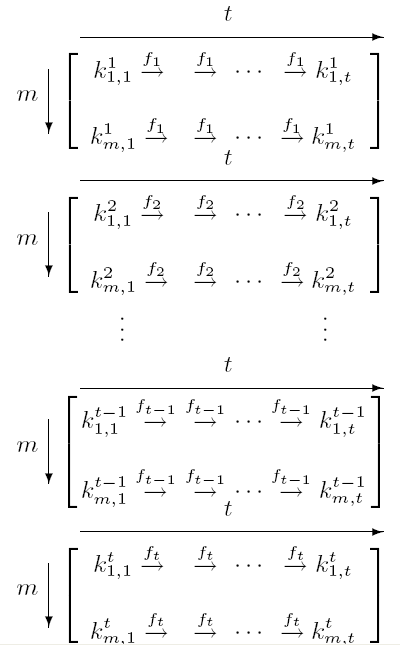
\includegraphics[width=3in]{./figures/hellman-tables.PNG}
	\caption{Structure of Hellman tables}	
	\label{fig:hellman-tables}
\end{figure}

The equations for creating the keys in the chain $j$ of table $i$ are shown below. The mapping function is denoted by $f_i$ and the reduction function by $R_j$.
\begin{align*}
& & K_{j,0} & = SP_j & & & &\\
1&. &K_{j,1} & = R_i(E_{K_{j,0}}(P)) & & & &\\
2&. &K_{j,2} & = R_i(E_{K_{j,1}}(P)) & & & &\\
& & &\vdots & & & &\\
(t-1)&. &K_{j,t-1} & = R_i(E_{K_{j,t-2}}(P)) & & & &\\
(t)&. &K_{j,t} & = R_i(E_{K_{j,t-1}}(P)) & & & &\\
& & EP_j & = K_{j,t} & & & &
\end{align*}

The time for precomputation is proportional to the number of computations that are done in all the tables, which is $mtr$. Hence, $P$ = $mtr$. Also, corresponding to each table, $m$ $(SP, EP)$ pairs exist in the hashtable. Hence, total number of pairs in the hashtables is $mr$, resulting in required precomputation memory of order $M$ = $mr$.\\

\noindent \textit{\textbf{Attack phase.}} During the attack phase, ciphertext $C$ is searched through each of the $r$ tables one by one. Let's consider the case in which $C$ is searched through a particular table $i$. 

First, $X$ is computed using the reduction function as, $X$ = $R_i(C)$. $X$ is then matched with the end points of the table. If $X$ matches with the end point $EP_{j}$ of the $j$'th chain, it means that the desired key lies in the $(t-1)$'th column of that chain. $SP_{j}$ is retrieved from the hashtable (for table $i$) and $(t-1)$ computations are perfomed using $f_i$ to obtain the key in the $(t-1)$'th column. We call this key $K_p$, $p$ standing for the possible key. If the ciphertext derived using $K_p$ is the same as $C$, then $K_p$ is the key we are looking for. Otherwise, we know that it is a case of false alarm. 

On the other hand, if $X$ does not match with any end point, $X$ is replaced with $f_i(X)$ and again matched with the end points. If there is a match, then the possible key appears in the $(t-2)$'th column. Just as before, $SP_{j}$ is retrieved from the hashtable and $(t-2)$ computations are performed of $F_i$ to obtain $K_p$. Occurence of false alarm is checked in the same way, confirming if $K_p$ is the desired key or not. 

$X$ is iteratively replaced by $f_i(X)$ for a maximum $(t-1)$ times, after which the same search is performed on the next table. If there is a match, and if it is not a false alarm, then the correct key is and the attack is terminated. 

In the worst case, $K$ is found after searching through all the tables. Searching a single table requires $t$ computations in the worst case. Hence, the attack time is proportional to $rt$. This implies that the order of the attack time is $T$ = $rt$.\\

\noindent \textit{\textbf{Tradeoff equation.}} We have derived the following relations for $M$ and $T$ so far, 
\begin{center}
$M = mr$\\
$T = rt$\\
\end{center}
Then, we have the table stopping rule,
\begin{center}
$mt^2 = 2^k$\\
\end{center}
Further, it is required that all the possible keys are covered in the Hellman tables. Since the number of keys computed during the precomputation is $mtr$, we require
\begin{align*}
mtr = 2^k
\end{align*}
From the last two equations, we have $r$ = $t$. Hence, the number of tables is equal to the length of each chain. Eliminating $m$ and $t$ from the relations for $M$ and $T$, we get the following tradeoff equation,
\begin{align}
\label{eq:hellman-block} M^{2}T = 2^k
\end{align}

\begin{table}[ht!]
\begin{center}
\begin{tabular}{c|c|c|c}
													&		Pre. time		& Pre. memory	& Attack time		 \\ \hline
Brute-force 							&		$-$		& $c$	 	& $2^k$		\\ \hline
Precomputed ciphertext		&		$2^k$	& $2^k$	& $c$		 	\\ \hline
TMTO using Hellman tables	&		$2^k$	& $M$ & $T$ 			\\
\end{tabular}
\end{center}
\caption{Performance of TMTO attack with Hellman tables}
\label{tab:hellman-tmto-comparison}
\end{table}

\noindent \textit{\textbf{Analysis.}} So how are Hellman tables better than a brute-force or precomputed ciphertext attack? Table \ref{tab:hellman-tmto-comparison} shows the order of precomputation time, precomputation memory and attack time for these three schemes. 

In the table, $c$ indicates a constant. The tradeoff attack reduces precomputation memory from $2^k$ in case of precomputed ciphertext attack to $M$. When compared with the brute-force attack, tradeoff attack reduces attack time from $2^k$ to $T$. Since both $M$ and $T$ are less than $2^k$ (from equation \ref{eq:hellman-block}), the tradeoff attack improves precomputation memory and attack time requirements. The only disadvantage of this attack, as also shown in the \mbox{table}, is in terms of the precomputation time. The tradeoff attack still requires precomputation time of the order of $2^k$.

\section{Hellman tables for stream ciphers}

Hellman tables for block ciphers have been used for mounting TMTO attacks on stream ciphers by Biryukov and Shamir in \cite{biryukov2000ctm}. Stream ciphers have a different working principle, and thus certain modifications in the original Hellman tables are proposed for them. 

Using Hellman tables an attacker can find the secret key $K$ if and only if the known plaintext $P$ is used in constructing the tables. Hence in a way, the tables are \emph{static} and cannot be re-used if a different plaintext and ciphertext pair for the same key are known. The tables can only be re-used if the same plaintext $P$ is later encrypted using a different key, say, during a different run of the protocol using the block cipher.

In addition, one of the important goals while constructing the tables for block ciphers is to cover all the possible keys. This is so because, a key can be found only when it is available in one of the tables. If the key does not exist, it can never be found as the ciphertext obtained using the key would not match in the tables. If the ciphertext matches, it would only turn out to be a key which gives the same ciphertext as the correct key. 

Tables for stream ciphers differ from those for block ciphers based on these grounds. Tables prepared for stream ciphers (as we have already seen in section \ref{sec:bg-keystream-attack}) are not bound to a particular plaintext. They are general tables with prefix to state mapping, and can be re-used any number of times for keystream from different keys. Once a match is found, the current state of the LFSR is determined and it is then reversed to obtain the initial state. After this, the specific initialization parameters are used in finding the key from the initial state.

Also, stream ciphers move through a number of internal states while generating the output keystream. If the attacker is able to find any one of these internal states, the initial state is recovered and thus the key. The attacker has knowledge of \emph{data}, which comprises of subsequences of the keystream or the prefix of each of the internal state that occurs while generating the keystream. Using this data, several attempts of matching the current state in the precomputed tables can be made, thus increasing the probability of finding the key. This flexibility is not available to an attacker breaking block ciphers, since the only data known there is the ciphertext $C$. 

Attacks taking into consideration the availability of data, in addition to time and memory, are called time-memory-data tradeoff attacks (or TMDTO attacks). TMDTO attacks are particularly suited to stream ciphers as a long keystream is available. Whereas in the case of block ciphers, we always have $D$ = $1$ representing the only available data $C$. Further, we describe the precomputation and attack phase for a TMDTO attack on stream ciphers.\\

\noindent \textit{\textbf{Precomputation phase.}} While attacking stream ciphers, the unknown part always is the current internal state and the known part is the prefix of the state. Before we discuss how the tables are organized, it is important to consider the number of states that are required to be covered by the tables, in order to have a high probability of a match. We have two set of states here; one, the states covered in the tables (number of such states is $P$) and two, the states covered while generating the keystream (the number of such states is $D$). According to equation \ref{eq:bday-paradox2}, in order to have a high probablity of a common state existing between these two sets, the product of the size of these sets must be greater than or equal to the size of the state space. 

Then we have the relation $PD$ $\geq$ $N$, where $N = 2^n$. If we ignore the greater than sign, we get the lower bound on $P$ and $D$, and we have $P$ = $N/D$. As compared to the tables for block ciphers, $P$ is reduced by a factor of $D$ for stream ciphers. According to \cite{biryukov2000ctm}, reduction in the number of precomputed states can be achieved by either reducing the number of states in each table, or by reducing the number of tables itself. From the relation $P$ = $mt$.$t$/$D$, either $mt$ must become $mt$/$D$ (thus reducing number of states in each table) or $t$ must become $t$/$D$ (thus reducing the number of tables). The authors argue that the former option is not a good idea. In that case, the tables would accomodate less states than the maximum states allowed in a table to prevent collisions. As a result, the latter option is chosen, and the number of tables is reduced by the factor $D$. This in turn creates a dependency between $t$ and $D$ such that $t \geq D$, as there should atleast be one table. Later in the section, we show how the dependency can be eliminated.

Thus for the precomputation phase, we have $t$/$D$ tables, each having $m$ chains with $t$ states each. The chains start with a random state $S_{j,0}$ (denoted by $SP_j$) indicating the first element in the j'th chain. The prefix for the starting state is computed, and a reduction function applied on the prefix to give the next state $S_{j,1}$. The prefix function is represented by $Prefix$ and the reduction function by $R$. Then, we have the following relation,
\begin{align*}
S_{j,1} = f_i(S_{j,0}) = R_i(Prefix(S_{j,0}))
\end{align*}  
\begin{figure}[ht!]
	\centering
		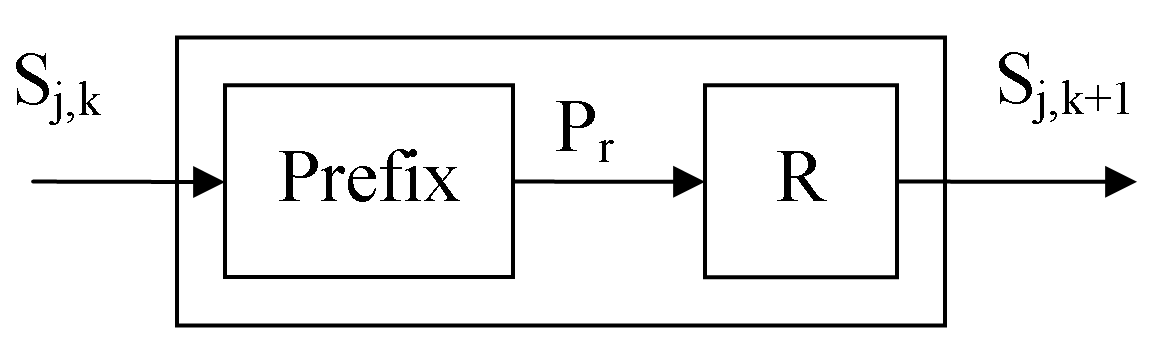
\includegraphics[width=3in]{./figures/mapping-function-stream.PNG}
	\caption{Mapping function for stream ciphers}	
	\label{fig:mapping-function-stream}
\end{figure}

The state $S_{j,1}$ is then used to compute $S_{j,2}$ and the process is repeated for $t$ such computations, at the end of which the last state $S_{j,t}$ is known. The mapping function $f_i$ is shown in the figure \ref{fig:mapping-function-stream} for such a transformation. The last state is referred to as end state and denoted by $EP_j$. In all, $m$ chains are created in this way as part of one table. The same is repeated for other tables but with different reduction functions, in order to avoid collision between different tables. 

The precomputation time $P$ for this phase is $mt^2/D$, as discussed before. Since the number of tables has reduced, the order of memory required to store the starting and end points of each chain also reduces. Hence we have, $M$ = $mt/D$.\\

\noindent \textit{\textbf{Attack phase.}} The attack phase for stream ciphers is similar to that for block ciphers. Every subsequence of the keystream is searched in all the tables. Each of the columns is checked for the possibility of the current state being present, and this repeated for each of the $t/D$ tables. In the worst case, the attack would require $t$ computations per table, for each prefix, which amounts to $t^2/D$ computations for each prefix. Hence the worst case attack time is of the order of $t^2$ and thus we have $T$ = $t^2$.\\

\noindent \textit{\textbf{Tradeoff equation.}} The tradeoff equation can be easily derived by eliminating the parameters $m$ and $t$ from the following three important equations,
\begin{align*}
M &= mt/D\\
T &= t^2\\
mt^2 &= N
\end{align*}
The tradeoff equation comes out to be,
\begin{align}
\label{eq:tmdto-hellman-stream} TM^2D^2 = N^2
\end{align}
  \\
\noindent \textit{\textbf{A general tradeoff equation.}} The tradeoff equation derived above is proposed in \cite{biryukov2000ctm} by Biryukov and Shamir. In the derivation of this equation, we have replaced the number of tables $r$ (the value of which is $t$ for block ciphers) with $r$ = $t/D$. The parameters $r$ and $t$ correspond to the precomputation phase whereas $D$ corresponds to the attack phase. Since the number of tables is such that $r \geq 1$, we have the condition that $D \leq t$. This creates a dependency of the attack phase parameter on the precomputation phase parameter. This dependency is particularly not helpful if we want to change $D$ frequently, for a fixed precomputation table. The precomputation phase in such a case would have to be carried out again with the new $D$ in consideration, before the attack could be mounted. 

Here, we describe a different and simpler form of the tradeoff equation, which uses the parameter $r$ in the precomputation phase without replacing it with $t/D$. Thus, if there are $r$ tables, with each table having $mt$ number of states, then the total number of states in the Hellman table structure is $mtr$. During the attack phase, $D$ states are traversed through, thus the product $mtr \times D$ must be $N$. Hence we have, 
\begin{align}
\label{eq:tmdto-hellman-general} mtr \times D = N
\end{align}
We call the equation \ref{eq:tmdto-hellman-general} as the general tradeoff equation for TMDTO attacks on stream ciphers using Hellman tables. Using this equation, the parameters $m$, $t$, $r$ and $D$ can be set independent of each other thus offering a greater flexibility while running the attack. Following these parameters, $T$ and $M$ can be calculated as follows.
\begin{align}
\label{eq:tmdto-hellman-general-memory} M &= mr\\
\label {eq:tmdto-hellman-general-time} T &= trD
\end{align}
In the next section results of the performance of Hellman tables for breaking HiTag2 are provided. The parameters used for these results are taken from the general tradeoff equation. Furthermore, the Biryukov and Shamir tradeoff equation is used for comparison with rainbow table in section \ref{sec:compare-hellman-rainbow}.

\section{Implementation and results}
\label{sec:hellman-table-impl}

The implementation of the Hellman tables for stream ciphers differs from the implementation of previously discussed TMTO attacks in certain ways. For every table a separate hashtable is constructed. This is because every table has its own reduction function. Each table is identified by a table number $i$ such that $1 \geq i \geq r$. The reduction function used for the table $i$ is shown in equation \ref{eq:reduction-function}, where $k$ represents a column in the chain $j$.

\begin{align}
\label{eq:reduction-function} S_{j,k+1} = f_i(S_{j,k}) = R_i(Prefix(S_{j,k})) = Prefix(S_{j,k}) \oplus i
\end{align}  

This ofcourse is a very simple reduction function and more complicated functions can be constructed. Though in the literal sense, this is not a reduction function since the input and output of the function are of same size which is 48 bits. This function is rather a permutation function and maps one element in the state space to another element in the same space. If prefixes of length 56 bits are used, then these 56 bits must be mapped to 48 bits of state. In this case, the terminology for the reduction function would be appropriate. But, we continue using the same name in the case of 48 bit prefixes in order to avoid creating new terms for special cases. 

The number of hashtables required is $r$ and the starting and end points of each table are stored in separate hashtables. In the implementation, we execute a separate program carry out the precomputation phase of the attack. This program computes the starting and end points for each table and stores them in an ASCII file on the local disk. The reason for doing this is that the precomputation takes hours to complete, for example for $P = 2^{33}$, the time taken is 13 hours. Hence, storing the tables in a file is a better idea instead of generating the precomputation tables each time the attack is executed.

The following steps are performed in sequence as part of the complete attack. 

\begin{enumerate}
\item The Hellman tables are created for given parameters $m,t,r$ and $D$, and stored in a file on the hard disk. This program is not part of the attack module.
\item The first step in the attack module is to prepare the hashtables by reading the file. The parameters from the file are matched with the parameters of the attack. If they are compatible then file reading process is continued. Otherwise the program terminates. The size of each hashtable prepared is $m$. The precomputation memory is as given by equation \ref{eq:tmdto-hellman-general-memory}. The time for precomputation $P$ is given by $mtr$.
\item Keystream is generated for the attack. The length of the keystream depends on value of $D$ chosen.
\item The attack is started. Each subsequence from the keystream is searched in the hashtable. The time for the attack is as given by equation \ref{eq:tmdto-hellman-general-time}. 
\end{enumerate}

The results of the attack for keys $K_2$ are shown below. 

%\begin{table}[ht!]
%\begin{center}
%\begin{tabular}{|c||c|c|c||c|c|c|c|c|}
%\hline
%Key & \multicolumn{4}{c||}{\textbf{$K_2$}} & \multicolumn{4}{c|}{\textbf{$K_3$}} \\ \hline \hline
%m																				&	$2^{16}$ 	&	$2^{14}$ 	&	$2^{16}$ 	&	$2^{14}$ 	&	$2^{16}$ 	&	$2^{14}$ 	&	$2^{16}$ 	&	$2^{14}$ 	 	\\ 
%t	  																		&	$2^{16}$ 	&	$2^{17}$ 	&	$2^{16}$ 	&	$2^{12}$	&	$2^{16}$ 	&	$2^{17}$ 	&	$2^{16}$ 	&	$2^{12}$	 	\\ 
%r	  																		&	$2^{1}$ 	&	$2^{1}$ 	&	$2^{2}$ 	&	$2^{6}$		&	$2^{1}$ 	&	$2^{1}$ 	&	$2^{2}$ 	&	$2^{6}$		 	\\ 
%D	  																		&	$2^{15}$ 	&	$2^{16}$ 	&	$2^{14}$ 	&	$2^{16}$	&	$2^{15}$ 	&	$2^{16}$ 	&	$2^{14}$ 	&	$2^{16}$	\\ \hline \hline
%M																				&	$2^{17}$ 	&	$2^{15}$ 	&	$2^{18}$ 	&	$2^{20}$ 	&	$2^{17}$ 	&	$2^{15}$ 	&	$2^{18}$ 	&	$2^{20}$ 	 	\\ 
%P	  																		&	$2^{33}$ 	&	$2^{32}$ 	&	$2^{34}$ 	&	$2^{32}$	&	$2^{33}$ 	&	$2^{32}$ 	&	$2^{34}$ 	&	$2^{32}$	 	\\ 
%T	  																		&	$2^{32}$ 	&	$2^{34}$ 	&	$2^{32}$ 	&	$2^{34}$	&	$2^{32}$ 	&	$2^{34}$ 	&	$2^{32}$ 	&	$2^{34}$	\\ \hline \hline
%Precomputation time for file (hours)		&	13 	 			&	6.5 			&						&	 					&	13 	 			&	6.5 			&						&	 					\\ \hline
%Time for attack	(hours)									&	6.7 			&	25.2			&	2.6 		 	&	5.1 			&	6					&	12				&						&						\\ \hline
%Number of times correct key is found 		&	2 				&	1					&	3 				&	1 				&	6					&	12				&						&						\\ \hline
%Time of first correct key (hours)				&	1.2 			&	24.0			&			 		 	&			 			&						&						&						&						\\ \hline
%Number of times false key is found			&	0 				&	1 				&	3 				&	3 				&	6					&	12				&						&						\\ \hline
%Number of false alarms									&	33009			&	66684			&	120				&	256				&	6					&	12				&						&						\\ \hline
%\end{tabular}
%\end{center}
%\caption{Results of TMDTO Hellman attack for $K_2$ and $K_3$}
%\label{tab:hellman-attack-results}
%\end{table}

\begin{table}[ht!]
\begin{center}
\begin{tabular}{|c||c|c|c|c|}
\hline
m																				&	$2^{16}$ 	&	$2^{14}$ 	&	$2^{16}$ 	&	$2^{14}$ 	\\ 
t	  																		&	$2^{16}$ 	&	$2^{17}$ 	&	$2^{16}$ 	&	$2^{12}$	\\ 
r	  																		&	$2^{1}$ 	&	$2^{1}$ 	&	$2^{2}$ 	&	$2^{6}$		\\ 
D	  																		&	$2^{15}$ 	&	$2^{16}$ 	&	$2^{14}$ 	&	$2^{16}$	\\ \hline \hline
M																				&	$2^{17}$ 	&	$2^{15}$ 	&	$2^{18}$ 	&	$2^{20}$ 	\\ 
P	  																		&	$2^{33}$ 	&	$2^{32}$ 	&	$2^{34}$ 	&	$2^{32}$	\\ 
T	  																		&	$2^{32}$ 	&	$2^{34}$ 	&	$2^{32}$ 	&	$2^{34}$	\\ \hline \hline
Precomputation time for file (hours)		&	13 	 			&	6.5 			&	XX				&	XX				\\ \hline
Time for attack	(hours)									&	6.7 			&	25.2			&	XX 			 	&	XX	 			\\ \hline
Number of times correct key is found 		&	2 				&	1					&	XX 				&	XX 				\\ \hline
Time of first correct key (hours)				&	1.2 			&	24.0			&	XX	 		 	&	XX	 			\\ \hline
Number of times false key is found			&	0 				&	1 				&	XX				&	XX				\\ \hline
Number of false alarms									&	33009			&	66684			&	XX				&	XX				\\ \hline
\end{tabular}
\end{center}
\caption{Results of TMDTO Hellman attack for $K_2$}
\label{tab:hellman-attack-results}
\end{table}

The following comments are made for these results.
\begin{enumerate}
\item 
\item 
\end{enumerate}
\chapter{Time-memory-data tradeoff using Rainbow table}
\label{chapter:tmdto-rainbow}

\paragraph{Summary}


\section{Rainbow table for block ciphers}
\label{sec:rainbow-block}

Rainbow table was introduced by Philippe Oechslin in \cite{oechslin:mfc}. Rainbow table (or rainbow chains, as called by the author) is a different way of precomputing data for the attack phase of a TMTO attack. Oechslin introduced rainbow table for block ciphers as an improvement over the Hellman tables. By using rainbow table, the attack time is expected to be reduced by a factor of $2$.

In Hellman tables, merging of chains within different tables is prevented by using different reduction functions for each table. However, collisions within the same table cannot be avoided completely. Though the number of elements in each table is restricted according to the table stopping rule, still there is no guarantee that collisions would not occur in the same table. This is due to the simple fact that birthday paradox is probabilistic in nature. Rainbow table solves this problem of collisions considerably.\\

\noindent \textit{\textbf{Precomputation phase.}} The rainbow table comprises of one huge table instead of $t$ tables, with $mt$ chains each having $t$ keys. The more interesting difference from Hellman tables is that instead of changing reduction function with table, reduction function is changed between columns in the rainbow table. If $SP_i$ is the starting point of a chain, then subsequent keys are computed by the functions \mbox{$f_1, f_2, \cdots, f_t$}, where $f_j(K) = R_j(E_{K}(P))$ for $1 \leq j \leq t$. This is shown in the following equations. 

\begin{align*}
& & K_{i,0} & = SP_i & & & &\\
1&. &K_{i,1} & = f_1(K_{i,0}) & & & &\\
2&. &K_{i,2} & = f_2(K_{i,1}) & & & &\\
& & &\vdots & & & &\\
(t-1)&. &K_{i,t-1} & = f_{t-1}(K_{i,t-2}) & & & &\\
(t)&. &K_{i,t} & = f_t(K_{i,t-1}) & & & &\\
& & EP_i & = K_{i,t} & & & &\\
\end{align*}

For every chain, the same sequence of mapping functions from $f_1$ to $f_t$ are used in computing subsequent keys. As usual, the starting and end points for each chain are stored in a hashtable, with the end points as the hashkey and the starting points as the hashvalue. The rainbow table is shown in figure \ref{fig:rainbow-table}.

\begin{figure}[ht!]
	\centering
		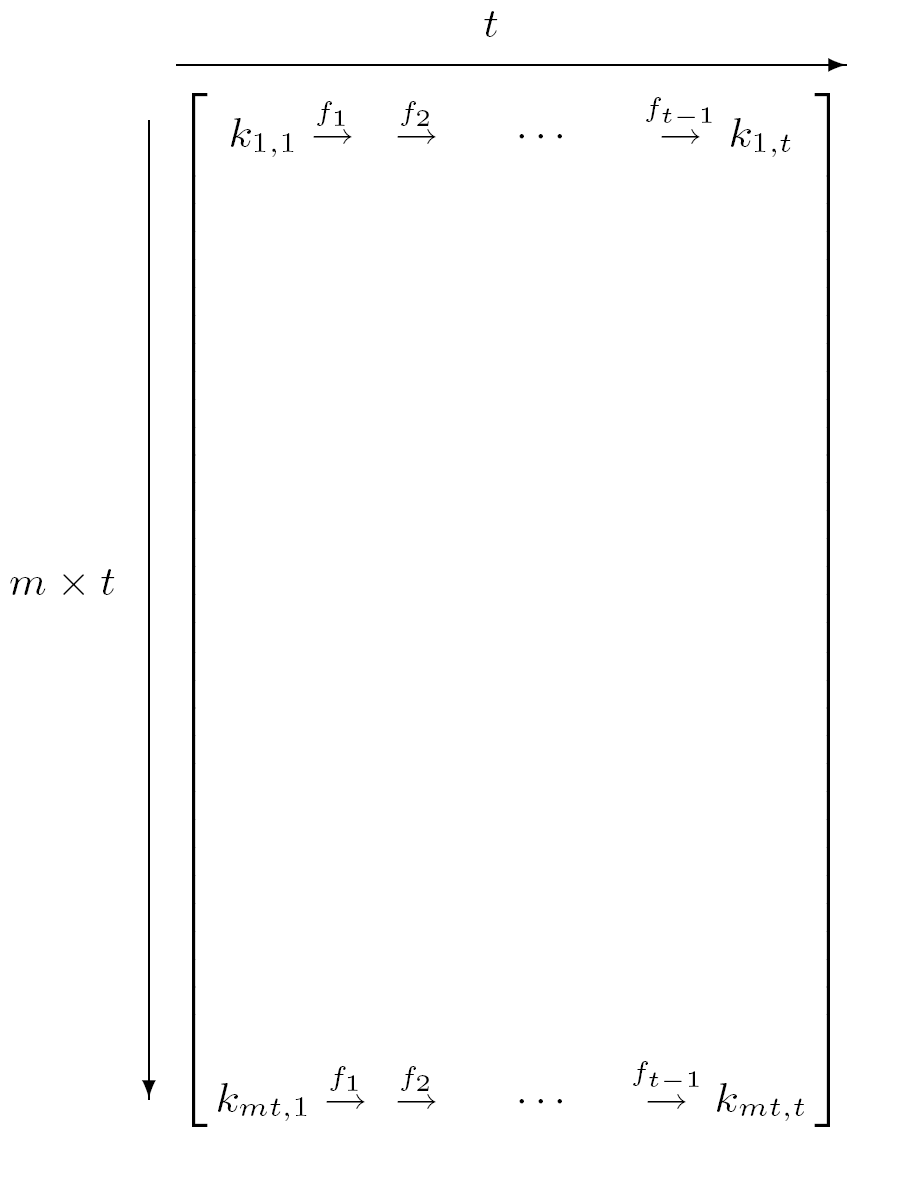
\includegraphics[width=3.5in]{./figures/rainbow-table.PNG}
	\caption{Rainbow table for block ciphers}	
	\label{fig:rainbow-table}
\end{figure}

The time for preparing the rainbow table is the same as the number of computations carried out. This is equal to $P$ = $mt \times t$ = $mt^2$. Also, the order of memory required for the hash table is $M$ = $mt$. \\

\noindent \textit{\textbf{Attack phase.}} The attack phase is a little more complicated as compared to that for Hellman tables. But, as we shall see, the number of computations required in the worst case, to find a match, is reduced by a factor of $2$. 

First, let's consider the possibility of the ciphertext appearing in the last column of the rainbow table. If this is the case, then an end point $EP_i$ would match with the reduction of the ciphertext $C$ which is $X$ = $R_t(C)$. Note that the reduction function for the $t$'th column is used here. If the match occurs, then $(t-1)$ computations are performed starting from the corresponding starting point $SP_i$, with the mapping function changing in each column. $K_{i,t-1}$ is then the required key, if it is not a false alarm. If the match does not occur, the number of operations (number of calls to any of the mapping functions $F_1$ to $F_t$) performed is $0$. 

So next, the possibility of $C$ appearing in the $(t-1)$'th column is explored. For this the value $X = F_{t}(R_{t-1}(C))$ is compared with the end points. If there is a match, then $(t-2)$ computations are performed from $SP_{i}$ using the mapping functions $F_1, F_2, \cdots, F_{t-2}$. The key $K_{i,t-2}$ computed is the required key. Otherwise, if there is no match, the number of operations performed is $1$.

This procedure is repeated for all the columns, until in a worst case scenario, $C$ happens to appear in the second column of the table. In such a case, we would iteratively call the mapping functions $F_2, F_3, \cdots, F_t$, thus amounting to $(t-1)$ operations, before $EP_j$ is matched. The total number of operations in the worst case scenario become, 

\begin{align*}
&= 0 + 1 + 2 + \cdots + (t-1)\\
&= t(t-1)/2\\
&\approx t^2/2
\end{align*}

The attack time then is of the order of $t^2/2$, thus $T$ = $t^2/2$.\\


\noindent \textit{\textbf{Tradeoff equation.}} Using the following equations, the tradeoff equation can be derived. 

\begin{align*}
M &= mt\\
T &= t^2/2\\
mt^2 &= N\\
\end{align*}

The tradeoff equation then comes to be,

\begin{align}
\label{eq:tmdto-rainbow-block} 2TM^2 &= N^2
\end{align}


\section{Rainbow table for stream ciphers and implementation}
\label{sec:rainbow-stream}

We derive a general tradeoff equation for attacks on stream ciphers using the rainbow table. An analysis similar to that done by Biryukov and Shamir for Hellman tables is described in section \ref{sec:compare-hellman-rainbow}. 

We start by saying that the number of chains in the rainbow table is $M$ and $t$ states exist in each chain. The total number of states in the table is $P = Mt$. Also, $D$ states occur during the attach phase. According to equation \ref{eq:bday-paradox2}, the product of $P$ and $D$ must satisfy the relation $P \times D \geq 2^n$. Considering the lower bound for $P$ and $D$, we have $P \times D = 2^n \Rightarrow MtD = 2^n$.
 
This relation allows us to select the parameters $M$, $t$ and $D$ in a manner such that the parameters determining the precomputation phase and those determining the attack phase are independent of each other. The time for searching a prefix in the hashtable is $t^2/2$. Hence, the total attack time for $D$ prefixes is $T = t^2D/2$. 

\noindent \textbf{\textit{Implementation}}. Since there is just one table storing the states in rainbow table, only one hashtable is required for storing the starting and end points. Just as in the implementation of Hellman tables for stream ciphers, we have implemented a separate program which computes this table and stores it on the local disk in the form of a ASCII file. The attack module reads the starting and end points from this file, and prepares the hashtable. Keystream of appropriate length depending on the value of $D$ is prepared for the attack. 

Following are the results of the attack for keys $K_1$ and $K_2$. 

\begin{table}[ht!]
\begin{center}
\begin{tabular}{|c||c|c||c|c|}
\hline
Key & \multicolumn{2}{c||}{\textbf{$K_1$}} & \multicolumn{2}{c|}{\textbf{$K_2$}} \\ \hline \hline
M																				&	$2^{24}$ 	&	$2^{24}$ 	&	$2^{24}$ 	&	$2^{24}$ 	\\ 
t	  																		&	$2^{8}$ 	&	$2^{9}$ 	&	$2^{8}$ 	&	$2^{9}$		\\ 
D	  																		&	$2^{16}$ 	&	$2^{15}$ 	&	$2^{16}$ 	&	$2^{15}$	\\ \hline \hline
P	  																		&	$2^{32}$ 	&	$2^{33}$ 	&	$2^{32}$ 	&	$2^{33}$	\\ \hline
T	  																		&	$2^{31}$ 	&	$2^{32}$ 	&	$2^{31}$ 	&	$2^{32}$	\\ \hline
Precomputation time for file (hours)		&	6 	 			&	12 				&	6					&	12 				\\ \hline
Time for preparing hashtable (seconds)	&	158				&	102				& 116				&	116				\\ \hline
Number of times false key is found			&	2 				&	1 				&	3 				&	3 				\\ \hline
Number of times correct key is found 		&	2 				&	3					&	3 				&	1 				\\ \hline
Number of false alarms									&	139				&	245				&	120				&	256				\\ \hline
Time for attack	(hours)									&	2.25 			&	5.10			&	2.56 		 	&	5.12 			\\ \hline
\end{tabular}
\end{center}
\caption{Results of TMDTO rainbow attack for keys $K_1$ and $K_2$}
\label{tab:rainbow-attack-results}
\end{table}

The following comments can be made based on the results from table \ref{tab:rainbow-attack-results}.
\begin{enumerate}
\item The time taken in creating the rainbow table (precomputation time for file) depends on $P$ or the number of states stored in the table. For $P$ = $2^{31}$, the time taken is around 6 hours, while for $P$ = $2^{32}$ it takes around 12 hours. 

\item The time for preparing the hashtable must be the same for all the cases (and both the keys), since $M$ is the same. But, we notice certain irregularity in the time, and this can be attributed to the machine on which the attack is run, as it is shared between various users. 

\item The correct key is found atleast once in all the cases, which is a good sign. Though, along with correct key, wrong keys are also being found in the attack. This must not be mistaken with the false alarms. These cases arise because of a prefix having more than one generating state or preimage. As a result, the prefix correctly exists in the rainbow table with the undesired state as its preimage. This state is found by the attack, resulting in a wrong key. We call such cases as false keys, and stress that they are different from false alarms. The only way of avoiding false keys is by increasing the length of prefix to 56 bits. As we have seen for TMTO keystream and tags attacks, 56 bits of prefix is sufficient in order to supress false keys. 

\item The time for attack is the total time taken for searching all the subsequences of the keystream. We have continued the attack even after the correct key is found, to know other results for the complete attack and the time taken for the same. For example, for the parameters in column 1 of $K_1$, the key is found for the first time in 595 seconds. The output from the attack is shown below.

\begin{lstlisting}[frame=tb]
Match!

Status:- D: 4800, Found column: 49
Found prefix: 196721643589477
Found Initial State: fe6e391b4972
Found Key: 52b49ea34972
TIME since starting attack: 595
\end{lstlisting}

It also says that the key is found in the 49'th column of the rainbow table, for the 4800'th subsequence of the keystream. 
\end{enumerate}




\section{Comparison of Hellman and rainbow table}
\label{sec:compare-hellman-rainbow}

In the case of Hellman tables, Biryukov and Shamir proposed changes to the table structure for block ciphers, in order to use them for stream ciphers. Just like Hellman tables, rainbow table has been proposed for block ciphers. Hence, they cannot be directly applied on stream ciphers. In the literature, we have not been able to find any considerable work in this direction. The paper by Erguler and Anarim is only work in this direction, to be best of our knowledge. Though 

The rainbow table discussed for block ciphers cannot be directly used for stream ciphers since we need to consider the data available for the attack. Clearly thus, the only change that is required is reducing the number of states in the rainbow table in proportion to the number of states in $D$. Let us say that $M$ chains exist in the table. Then the number of states in the table is $Mt$. If the number of states is to be reduced, then either $M$ or $t$ or both would be reduced. We have identified these possibilities in the following table. 


As we can see, if $M$ is reduced to $M/D$, then $T$ becomes $t^2D/2$, which is a very large value as compared to $t^2$ for Hellman tables. Also, if we decrease $t$ to $t/D$, then $M$ increases by factor $D$ as compared again with the Hellman tables.The only optimum value of both $M$ and $t$ is achieved in the third case. In this case, $M$ is increased by a factor of $\sqrt{D}$, while we can see that $T$ reduces by 2. Hence, this configuration of the rainbow table provides a good way of comparison with the performance of Hellman tables. 


\begin{align}
\label{eq:tmdto-rainbow-stream} 2TM^2D^2 &= N^2
\end{align}
\chapter{Conclusion}

\section{Comparison of Hellman and rainbow table}
\label{sec:compare-hellman-rainbow}

To use Hellman tables with stream ciphers, Biryukov and Shamir proposed changes in the table structure by taking $D$ into consideration. The original idea of rainbow table has been proposed for block ciphers and thus similar changes in the table structure are needed to use them with stream ciphers. The paper \cite{erguler2005nct} by Erguler and Anarim is the only work in this direction, to be best of our knowledge. The tradeoff described in the paper was designed independently by us. Only later it came to our knowledge that the idea has already been published by Erguler and Anarim.

With the availability of $D$, the number of states in the rainbow table can be reduced by the factor $D$. The number of states existing in the rainbow table is $Mt$ \footnote{The parameters $M$ and $t$ here represent the original rainbow table, and are not related with the parameters described in the general tradeoff equation in previous section}. Then either $M$ or $t$ or both should be reduced. These three possibilities are identified in the following table. 

\begin{table}[ht!]
\begin{center}
\begin{tabular}{|c||c||c c c|}
\hline
			& Biryukov-Shamir approach 	& \multicolumn{3}{c|}{Approach for rainbow tables}					\\ \hline \hline
M			&	M/D		&	M/D				&	M						& $M/\sqrt{D}$	\\
t			&	t			&	t					&	t/D					& $t/\sqrt{D}$	\\ \hline \hline
P			&	Mt/D	&	Mt/D			&	Mt/D				& Mt/D					\\ 
T			&	$t^2$	&	$t^2D/2$	&	$t^2/2D$		& $t^2/2$				\\ \hline
\end{tabular}
\end{center} 
\caption{Options for modifying parameters $M$ and $t$ for rainbow tables}
\label{tab:parameters-rainbow-table}
\end{table}

The first case for rainbow tables is reducing $M$ to $M/D$. Though memory required for the attack reduces, the time for the attack increases considerably to $t^2D/2$. It is interesting to note that for Hellman tables, the attack time depends on both $t$ and the number of tables. So, if $M$ is decreased, the number of tables decreases, thus reducing the attack time to $t^2$. On the other hand, for rainbow tables, the attack time depends just on the length of each chain. Hence, reducing the memory does not reduce the time for the attack.

In the next case, we reduce $t$ to $t/D$. The problem with this option is the increased memory requirement which is $M$. 

The third option is a middle way between the first two options. We reduce both $M$ and $t$ by a factor of $\sqrt{D}$. The attack time now becomes ${(t/\sqrt{D})}^2/2 \times D$ = $t^2/2$. As we see, this makes it comparable to the attack time for Hellman tables. Rainbow tables provide the same advantage for stream ciphers with this option, as they do for block ciphers i.e.~they reduce the attack time by a factor of 2. 

But, the memory requirement is $\sqrt{D}$ times greater than that for Hellman tables. This is a disadvantage of using rainbow table with these parameters.

Let us denote the memory requirement and the number of states in each chain by $M'$ and $t'$ for the modified rainbow table. Then we have $M' = M/\sqrt{D}$ and $t' = t/\sqrt{D}$. Replacing these values in the general tradeoff equation \ref{eq:general-rainbow-stream}, we get the following tradeoff equation.
\begin{align}
\label{eq:tmdto-rainbow-stream} 2TM^2D^2 &= N^2
\end{align}
For comparing the performance of Hellman and rainbow tables using their tradeoff equations, we select the following values of the required parameters based on the third option discussed above. 

\begin{table}[ht!]
\begin{center}
\begin{tabular}{|c|c c||c c|}
\hline
			& \multicolumn{2}{c||}{$M = 2^{32}$, $t = 2^{16}$, $D = 2^{14}$} 	& \multicolumn{2}{c|}{$M = 2^{31}$, $t = 2^{17}$, $D = 2^{16}$}	\\ \hline \hline
			&	Hellman				&	Rainbow					&	Hellman					& Rainbow				\\ \hline \hline
m			&	$2^{16}$			&		-							&	$2^{14}$				& 	-						\\ \hline 
t			&	$2^{16}$			&	$2^{9}$					&	$2^{17}$				& $2^{9}$				\\ \hline 
r			&	$2^{2}$				&		-							&	$2^{1}$					& 	-						\\ \hline 
M			&	$2^{18}$			&	$2^{25}$				&	$2^{15}$				& $2^{23}$			\\ \hline 
P			&	$2^{34}$			&	$2^{34}$				&	$2^{32}$				& $2^{32}$			\\ \hline 
T			&	$2^{32}$			&	$2^{31}$				&	$2^{34}$				& $2^{33}$			\\ \hline 
\end{tabular}
\end{center} 
\caption{Parameters for comparison of Hellman and rainbow table}
\label{tab:parameters-comparison}
\end{table}

The comparison of the results obtained using these parameters for Hellman and rainbow tables is shown in table \ref{tab:comparison-results-hellman-rainbow}.

\begin{table}[ht!]
\begin{center}
\begin{tabular}{|c|c c||c c|}
\hline
																				&	H							&	R								&	H								& R							\\ \hline \hline
M																				&	$2^{18}$			&	$2^{25}$				&	$2^{15}$				& $2^{23}$			\\ \hline 
m																				&	$2^{16}$			&		-							&	$2^{14}$				& 	-						\\ \hline 
t																				&	$2^{16}$			&	$2^{9}$					&	$2^{17}$				& $2^{9}$				\\ \hline 
r																				&	$2^{2}$				&		-							&	$2^{1}$					& 	-						\\ \hline 
P																				&	$2^{34}$			&	$2^{34}$				&	$2^{32}$				& $2^{32}$			\\ \hline 
D																				&	$2^{14}$			&	$2^{14}$				&	$2^{16}$				& $2^{16}$			\\ \hline \hline
T																				&	$2^{32}$			&	$2^{31}$				&	$2^{34}$				& $2^{33}$			\\ \hline \hline
Precomputation time for file (hours)		&	XX 	 					&	29.5						&	6.5							&	7.4						\\ \hline
Time for attack	(hours)									&	XX 	 					&	2.3							&	25.2						&	10.1					\\ \hline
Number of times correct key is found 		&	XX 	 					&	2 							&	1 							&	1 						\\ \hline
Time of first correct key (hours)				&	XX 	 					&	0.01						&	24							&	0.8						\\ \hline
Number of times false key is found			&	XX 	 					&	2 							&	1 							&	1 						\\ \hline
Number of false alarms									&	XX 	 					&	286							&	66684						&	247						\\ \hline
\end{tabular}
\end{center} 
\caption{Comparison of results of TMDTO attacks}
\label{tab:comparison-results-hellman-rainbow}
\end{table}

\section{Concluding remarks}

In this thesis, we have implemented various tradeoff attacks on the HiTag2 stream cipher and presented the results of the same. Babbage and Golic first proposed how a time-memory tradeoff attack can be implemented on stream ciphers. In block ciphers, encryption is performed on a block of plaintext yielding a block of ciphertext. The goal in attacks on block cipher is always to successfully invert the transformation from the input to output block. In stream ciphers, this transformation was not understood until Babbage and Golic proposed that the transformation from state to the prefix must be inverted to break the stream cipher, as this determines an internal state. 

This idea by Babbage and Golic has been used in all the attacks that we implemented. The first attack assumed the availability of very long keystream from the cipher, thus huge number of internal states and corresponding prefix. The second attack assumed several shorter keystreams. In the third attack Hellman tables were used to precompute states, while in the fourth attack rainbow table was used for the same purpose. 

In the first two attacks, the tradeoff equation contains the parameters $M$ and $T$. In these attacks, the hashtable stores each of the (state, prefix) pairs computed during the precomputation. Hence, the order of memory requirement and precomputation time are equal. Similarly, the attack time depends only on the keystream available, as the time taken to search one prefix in the hashtable is constant. Though we do not see $D$ in the equation, it is clear how $D$ affects the tradeoff through $T$.

In the last two attacks, three parameters $M$, $T$ and $D$ appear in the tradeoff equation. In these attacks, the hashtable does not store all the precomputed elements, which leads to $P$ being less than $M$. As a result, $P$ does not only depend on $M$ but also on the factor $t$. In addition, the time for the attack is no more equal to $D$ and depends on an additional factor $t$. 

In all attacks though, the main idea has been about two different sets of states and finding a collision between them; one set computed during the precomputation phase and the other occuring during the attack phase, represented by $P$ and $D$ respectively. The birthday paradox helps in deriving the relation $P \times D \geq N$, which is used as the basis for all the attacks. 

% performance of tmto and tmdto attacks? identify change in parameters?


\section{Future work}

The four attacks have been carried out in limited time, hence there is a lot of scope for improving the efficiency of the attacks. The last two attacks especially were time consuming, which resulted in a less number of results for them. Also there are many open research possibilities on the ideas concerned with these attacks. All of this is summarized in the following points. 

\begin{enumerate}
\item We have seen the results of the first two attacks with prefix length of 56 bits. These results indicate that 56 bits is the desirable length of prefix. The two TMDTO attacks have been implemented with just 48 bits of prefix, and it is expected that with 56 bits of prefix, the results would be more sound. Hence, more experiments need to be carried out with the longer prefix length.

\item Once we consider 56 bits of prefix for the TMDTO attacks, a reduction function needs to be in place. In our implementation, the reduction function is a simple xor of the 48 bit prefix with the table number (in Hellman tables) or the function number (in rainbow table), as the prefix length and state size are same. According to \cite{email-karsten}, the reduction function must be such that all the 56 bits of prefix must be accounted for computing the 48 bits of next state. 

\item We still need to analyze how the number of collisions in the Hellman and rainbow table can be reduced. Nohl provides us some insight into o
\end{enumerate}

\bibliography{thesis}
\bibliographystyle{plain}
\addcontentsline{toc}{chapter}{\bibname}

\appendix
\chapter{Check for irreducible polynomial in Matlab}
\label{app:irreducible-polynomial}
Following is the input to Matlab.
 
\begin{lstlisting}[frame=tb]
p = [1,0,1,1,0,0,1,1,1,0,0,0,0,0,0,0,1,0,0,0,0,0,1,1,0,
		0,1,0,0,0,1,0,0,0,0,0,0,0,0,0,0,1,1,1,0,0,1,1,1]

p =  Columns 1 through 12

     1  0  1  1  0  0  1  1  1  0  0  0

  	 Columns 13 through 24

     0  0  0  0  1  0  0  0  0  0  1  1

     Columns 25 through 36

     0  0  1  0  0  0  1  0  0  0  0  0

     Columns 37 through 48

     0  0  0  0  0  1  1  1  0  0  1  1

     Column 49

     1
\end{lstlisting}

No decisive output is observed from Matlab for approximately 24 hours. Hence, program is terminated.

\chapter{HiTag2 library}
\label{app:hitag2-lib}
Following is the implementation of the HiTag2 stream cipher in C language.
 
\begin{lstlisting}[frame=tb]
#include<stdio.h>
#include "common.h"
#include "hitag2.h"

static u64 hitag2_output(const u64 x)
{
	u64 i5;

	i5 = ((ht2_f4a >> i4 (x, 1, 2, 4, 5)) & 1)* 1
	   + ((ht2_f4b >> i4 (x, 7,11,13,14)) & 1)* 2
	   + ((ht2_f4b >> i4 (x,16,20,22,25)) & 1)* 4
	   + ((ht2_f4b >> i4 (x,27,28,30,32)) & 1)* 8
	   + ((ht2_f4a >> i4 (x,33,42,43,45)) & 1)*16;

	return (ht2_f5c >> i5) & 1;
}

u64 hitag2_init(const u64 key, const u32 serial, const u32 IV)
{
	u32 i = 0;
	u64 x = ((key & 0xFFFF) << 32) + serial;

	for (i = 0; i < 32; i++)
	{
		x >>= 1;
		x += (u64) (hitag2_output(x) ^ (((IV >> i) ^ 
		(key >> (i+16))) & 1)) << 47;
	}
	return x;
}

static u64 hitag2_round(u64 *state)
{
	u64 x = *state;

	x = (x >>  1) +
	 ((((x >>  0) ^ (x >>  2) ^ (x >>  3) ^ (x >>  6)
	  ^ (x >>  7) ^ (x >>  8) ^ (x >> 16) ^ (x >> 22)
	  ^ (x >> 23) ^ (x >> 26) ^ (x >> 30) ^ (x >> 41)
	  ^ (x >> 42) ^ (x >> 43) ^ (x >> 46) ^ (x >> 47)) & 1)
	  << 47);

	*state = x;
	return hitag2_output(x);
}

static u64 hitag2_byte(u64 * x)
{
	u64 i;
	u64 c;

	for (i = 0, c = 0; i < 8; i++) 
		c += (u64) hitag2_round(x) << (7 - i);
	return c;
}

u64 hitag2_prefix(u64 * x, u32 bits)
{
	u64 i;
	u64 prefix = 0;

	for (i = 0; i < (bits/8); i++)
	{
		prefix += 
		(u64) hitag2_byte (x) << ((bits/8) - 1 - i)*8;
	}
	return prefix;
}

void hitag2_prev_state(u64 *state)
{
	u64 x = *state;

	x = (x <<  1) +
	(((x >>  47) ^ (x >>  1) ^ (x >>  2) ^ (x >>  5)
	  ^ (x >>  6) ^ (x >>  7) ^ (x >> 15) ^ (x >> 21)
	  ^ (x >> 22) ^ (x >> 25) ^ (x >> 29) ^ (x >> 40)
	  ^ (x >> 41) ^ (x >> 42) ^ (x >> 45) ^ (x >> 46)) & 1);

	*state = x & 0xFFFFFFFFFFFFULL;
}

void hitag2_next_state(u64 *state)
{
	u64 x = *state;

	x = (x >>  1) +
	 ((((x >>  0) ^ (x >>  2) ^ (x >>  3) ^ (x >>  6)
	  ^ (x >>  7) ^ (x >>  8) ^ (x >> 16) ^ (x >> 22)
	  ^ (x >> 23) ^ (x >> 26) ^ (x >> 30) ^ (x >> 41)
	  ^ (x >> 42) ^ (x >> 43) ^ (x >> 46) ^ (x >> 47)) & 1) 
	  << 47);

	*state = x;
}

u64 hitag2_find_key(u64 initial_state, const u32 serial, 
	const u32 IV)
{
	u64 last_bit = 0;
	u64 key = 0;
	u64 state = 0;
	s32 i = 31;

	state = initial_state;

	for (i = 31; i >= 0; i--)
	{
		last_bit = (state >> 47);

		key = key + (((last_bit ^ hitag2_output(state) ^ 
			(IV >> i)) & 1) << (i + 16));
		state = (state << 1) + (u64) ((serial >> i) & 1);
	}
	
	key = key ^ ((state >> 32) & 0xFFFF);
	return key;
}
\end{lstlisting}

\chapter{C Program to check period of random number generator}
\label{app:random-function}

The following listing contains the C program for checking the period of a random generator function. The function \textit{get\_random\_2} introduced in section \ref{sec:keystream-attack-impl} is used in the listed program. However, this can be changed to check the desired function. 

The implementation checks for repetition of three consecutive random numbers. We believe checking three numbers is sufficient to identify a the repeating sequence.\\

\begin{lstlisting}[frame=tb]
#include <stdio.h>
#include <stdlib.h>
#include <time.h>
#include <math.h>

#define u8			unsigned char
#define u32			unsigned int
#define u64			unsigned long long

int main(void)
{
	time_t seconds;
	u64 runtime = 0;
	u64 i = 0;
	u64 first_random = 0;
	u64 second_random = 0;
	u64 third_random = 0;

	u64 random = 0;

	time(&seconds);
	srand(seconds);

	runtime = pow(2,32);
	
	first_random = get_random_2(48);
	second_random = get_random_2(48);
	third_random = get_random_2(48);
	
	printf("\nFirst random number: %llx", first_random);
	printf("\nSecond random number: %llx", second_random);
	printf("\nThird random number: %llx", third_random);
	
	for(i = 0; i < runtime; i++)
	{
		random = get_random_2(48);	
		
		if(random == first_random)
		{
			printf("\n\n Reoccurence: %llu\n", i);
			random = get_random_2(48);

			if(random == second_random)
			{
				random = get_random_2(48);
				
				if(random == third_random)
				{
				 printf("\n\n Repetition of 
				     random number! 
				     Period: %llu\n", i);
				 break;
				}
			}
		}
	}
}			
\end{lstlisting}



\end{document}
